\chapter{Экспериментальное исследование и оценка эффективности}
\label{chap:experiments}

В данной главе представлены результаты экспериментального исследования разработанной навигационной системы на реальном дорожном графе Московской агломерации. Приводятся характеристики испытательного стенда, методология тестирования, а также подробный анализ влияния низкоуровневых оптимизаций, безблокировочных структур данных и архитектурных решений на производительность вычислительного ядра и качество регулирования трафика.

\section{Методология тестирования и анализ эффективности алгоритмов поиска пути}

\subsection{Методология проведения экспериментов и исследуемые конфигурации}
\label{subsec:experiment_methodology}
Экспериментальное исследование проводилось на аппаратном стенде следующей конфигурации:
\begin{itemize}
    \item Центральный процессор: AMD Ryzen $5$ 5600H (микроархитектура Zen $3$, $6$ физических ядер, $12$ логических потоков SMT, базовая частота $3{,}3$~ГГц, максимальная частота $4{,}2$~ГГц, объединенный L3-кэш $16$~МБ);
    \item Оперативная память: $32$~ГБ DDR4 (частота $3200$~МГц, тайминги CL22, двухканальный режим);
    \item Накопитель: NVMe SSD $500$~ГБ (скорость последовательного чтения до $3100$~МБ/с);
    \item Операционная система хоста: Arch Linux (ядро Linux 6.19.14-zen1 с планировщиком PREEMPT\_DYNAMIC) \cite{containers_cmu};
    \item Среда сборки и выполнения: контейнер Docker на базе официального образа \texttt{gcc:14} (Debian Trixie) с флагами оптимизации компилятора \texttt{-O2 -march=native -mavx2 -flto} \cite{fog_optimizing_cpp, evtikhov2020hpc}.
\end{itemize}

Методология тестирования базировалась на генерации синтетической нагрузки, соответствующей утреннему часу пик в мегаполисе:
\begin{enumerate}
    \item В качестве картографической основы использован субграф Московской агломерации. Граф содержит $582$~тыс. узлов и $1~460$~тыс. ориентированных ребер.
    \item Сгенерировано $500$ случайных пар начальных и конечных вершин для расчета маршрутов.
    \item Все исследуемые алгоритмы поиска пути реализованы в рамках единой кодовой базы с применением низкоуровневых оптимизаций: векторизации приоритетных очередей и оптимизированной раскладки графа в памяти для минимизации промахов кэша. В качестве базовой конфигурации для сравнения принят классический алгоритм Дейкстры на двоичной куче.
\end{enumerate}

Для проведения сравнительного анализа исследованы следующие кандидаты алгоритмов поиска кратчайших путей и приоритетных очередей.

Исследованные алгоритмы поиска пути:
\begin{itemize}
    \item Алгоритм Дейкстры \cite{cherkassky1994shortest};
    \item Двунаправленный алгоритм Дейкстры \cite{goldberg2005external};
    \item Алгоритм A* \cite{goldberg2004alt};
    \item Алгоритм ALT \cite{goldberg2004alt}.
\end{itemize}

Исследованные очереди приоритетов \cite{outerloop_heap}:
\begin{itemize}
    \item Древесные кучи на основе сравнений:
    \begin{itemize}
        \item двоичная куча (в легендах графиков~-- \texttt{2-ary}) \cite{biggar_sorting};
        \item многоарные кучи (\texttt{4-ary}, \texttt{8-ary} и \texttt{16-ary}) \cite{kusswurm2014modern};
    \end{itemize}
    \item Распределительные очереди на базе корзин или разрядов:
    \begin{itemize}
        \item корзиночная очередь (\texttt{bucket}) \cite{ahuja1990faster};
        \item поразрядная куча (\texttt{radix}) \cite{ahuja1990faster};
        \item дельта-очередь (\texttt{delta}) \cite{meyer2003delta}.
    \end{itemize}
\end{itemize}

Для оценки эффективности представленных конфигураций в разработанной системе динамического регулирования транспортных потоков проведено многокритериальное исследование. На первом этапе анализируется влияние приближенных очередей и взвешенных эвристик ($w = 1{,}15$ для алгоритма $A^*$ и поиска по ориентирам $ALT$) на геометрическую точность получаемых маршрутов. На втором этапе исследуются низкоуровневые аппаратные характеристики операций вставки и извлечения из очередей на целевой архитектуре хоста. На финальном этапе результаты точности и аппаратной сложности сопоставляются в рамках интегрального анализа пропускной способности ядра маршрутизации.

\subsection{Анализ точности эвристического поиска кратчайших путей и влияние приближенных очередей}
\label{subsec:accuracy_analysis}

Важнейшим аспектом внедрения оптимизированных алгоритмов и приближенных структур данных является оценка их влияния на точность получаемых маршрутов. Эксперименты проводились при коэффициенте взвешенности эвристики $w = 1{,}15$, что согласно разделу \ref{sec:mathematical_model}, сокращает время расчета в $2{,}5$--$3{,}2$ раза по сравнению со строго оптимальным поиском ($w = 1{,}0$) при сохранении средней погрешности в пределах $1{,}3\%$ для точных куч.

Относительная погрешность веса пути для каждого тестируемого запроса рассчитывается как процентное отклонение веса пути, найденного исследуемой конфигурацией, от эталонного веса кратчайшего пути, полученного алгоритмом Дейкстры на двоичной куче:

\begin{equation}
    \varepsilon_i = \frac{|W_{algo}(i) - W_{Dijkstra}(i)|}{W_{Dijkstra}(i)} \times 100\%
\end{equation}
\where{
    $\varepsilon_i$ & относительная погрешность веса пути на $i$-м запросе; \\
    $W_{algo}(i)$ & вес пути, найденный исследуемым алгоритмом для $i$-й задачи; \\
    $W_{Dijkstra}(i)$ & эталонный вес кратчайшего пути, рассчитанный классическим алгоритмом Дейкстры на двоичной куче.
}

Для интегрального анализа точности использовались следующие показатели:
\begin{enumerate}
    \item Средняя относительная погрешность~-- усредненное значение $\varepsilon_i$ по всему тестовому набору запросов для каждого интервала сложности.
    \item Максимальная относительная погрешность~-- наибольшее зафиксированное отклонение веса пути среди тестовых задач.
    \item Доля точных совпадений~-- процент задач, для которых найденный вес пути строго равен эталонному ($\varepsilon_i = 0{,}0\%$).
\end{enumerate}

Результаты оценки точности для различных комбинаций алгоритмов и очередей приоритетов визуализированы на рисунке \ref{fig:accuracy_comparison}. На графике сопоставлены показатели всех исследованных типов очередей приоритетов для каждого из четырех рассматриваемых алгоритмов поиска пути.

\begin{figure}[htbp]
    \centering
    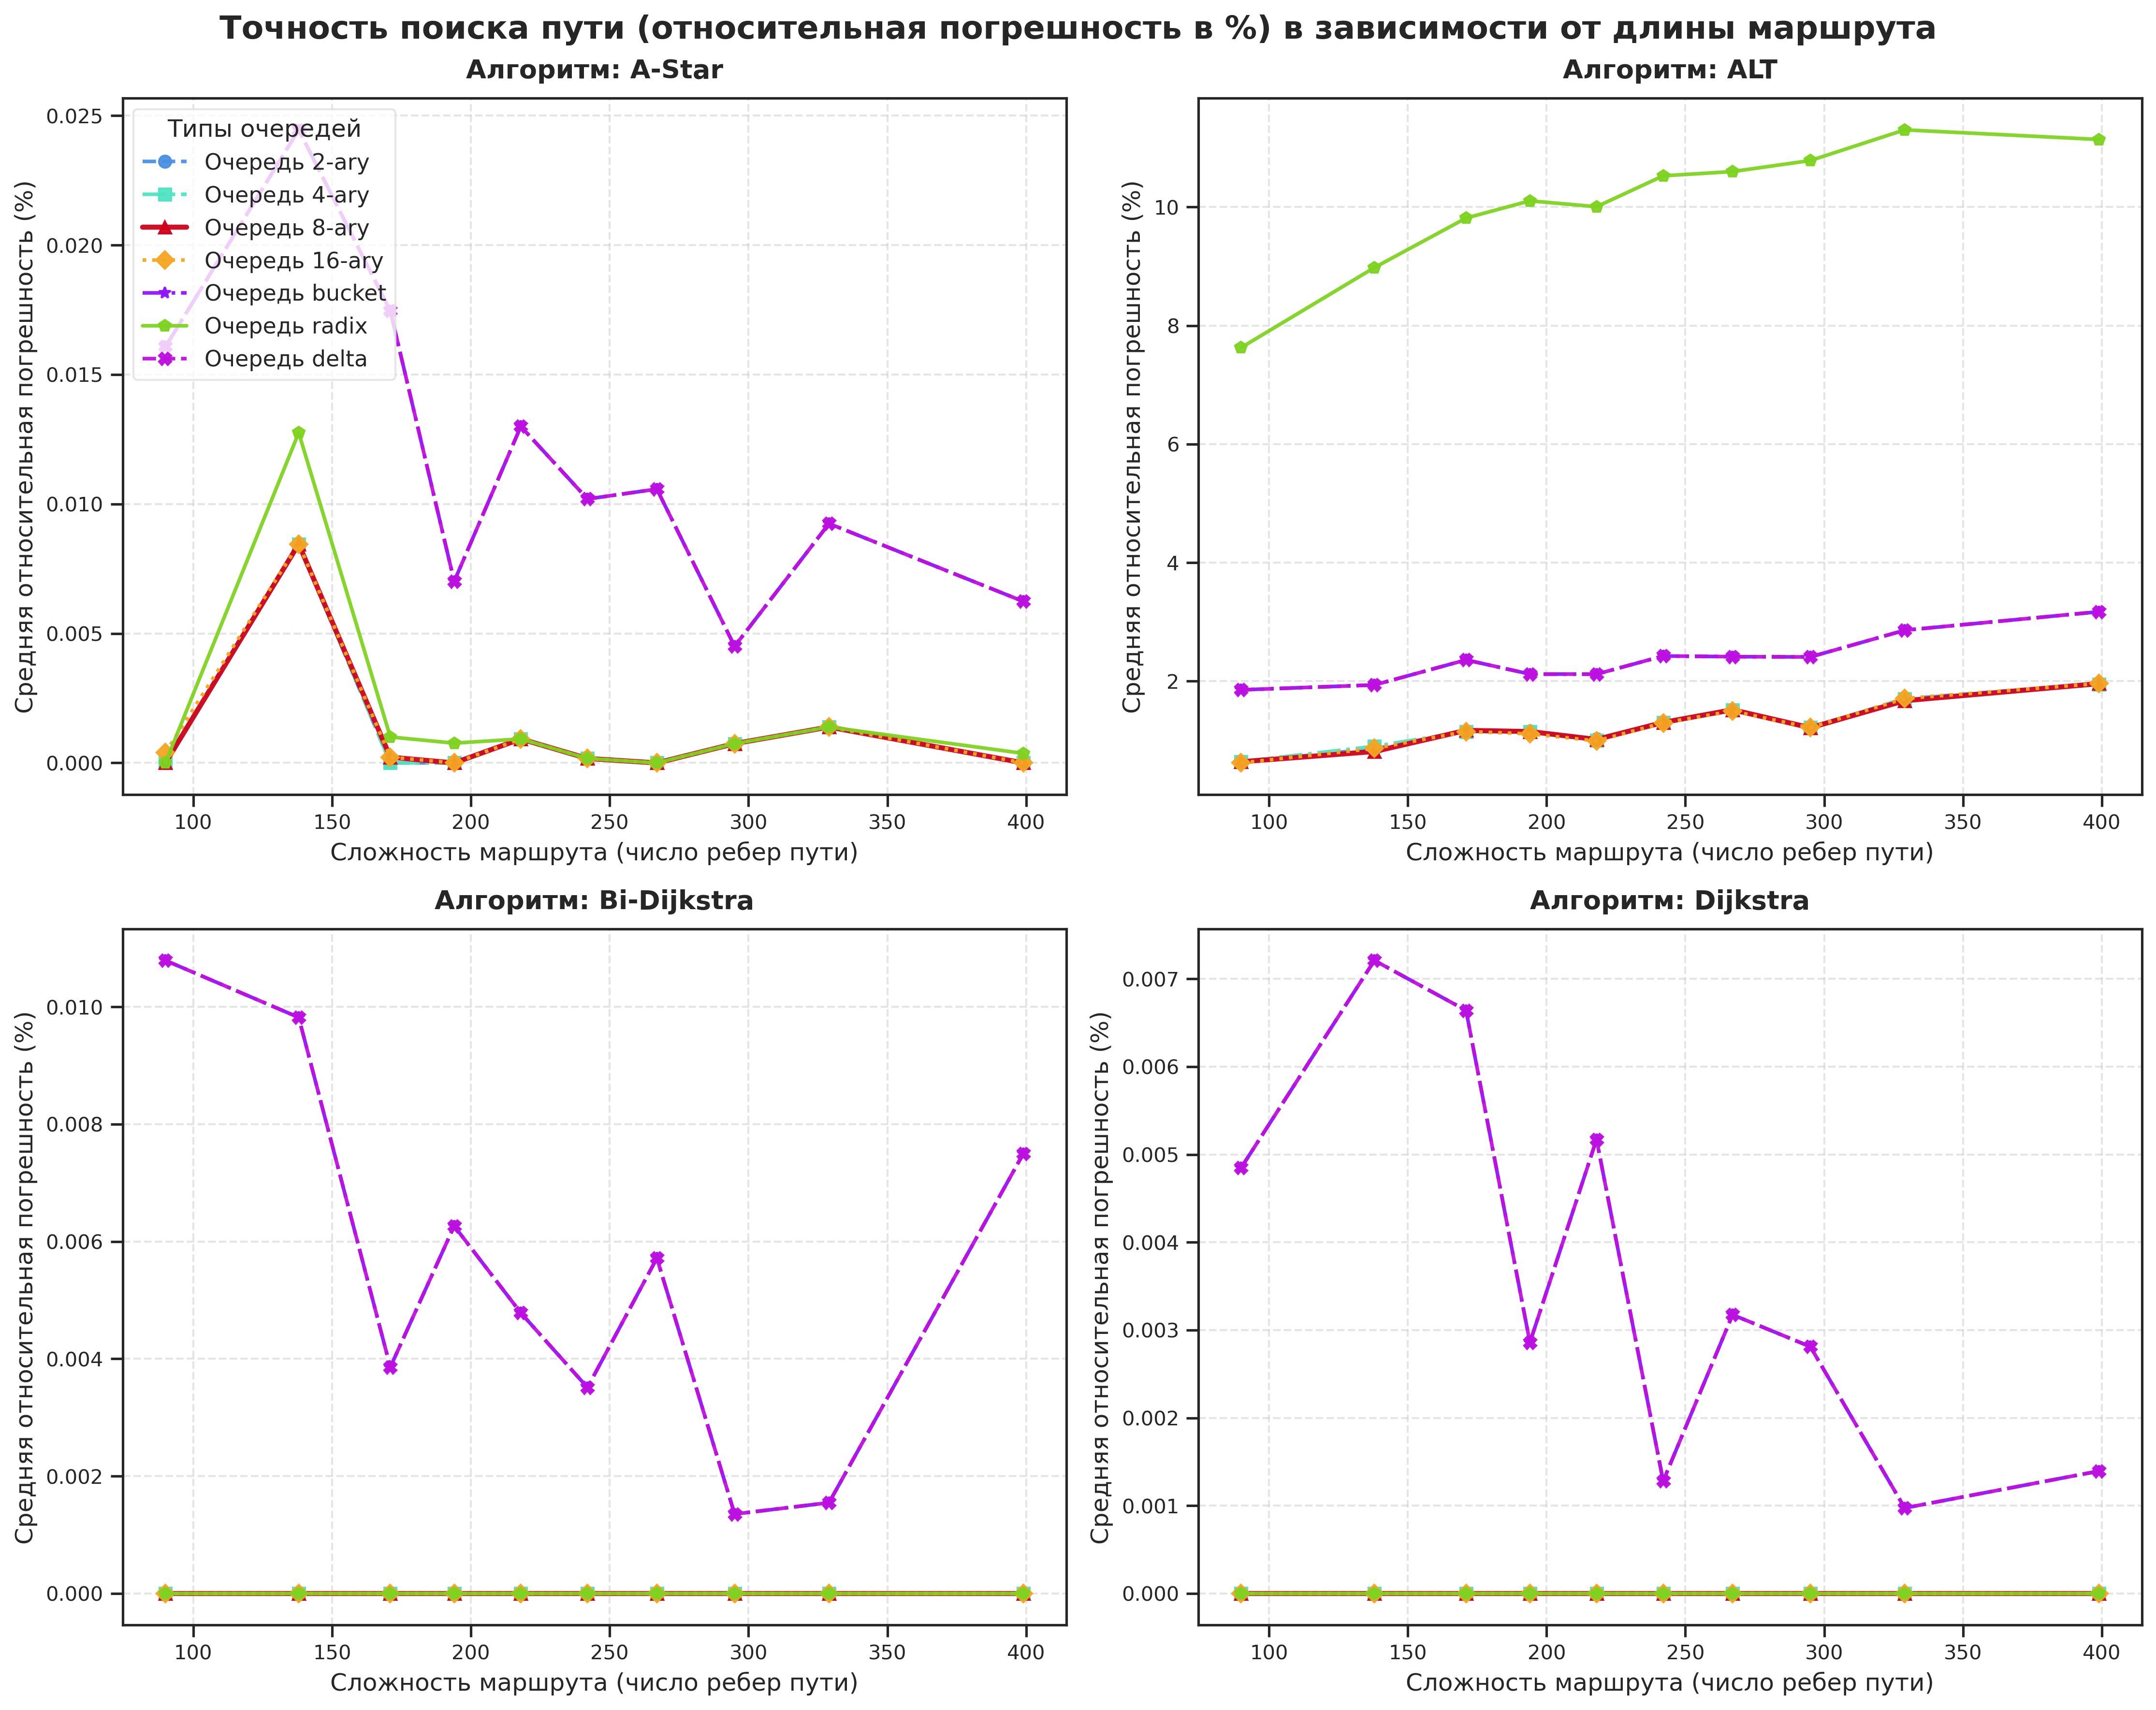
\includegraphics[width=\linewidth,keepaspectratio]{assets/images/accuracy_comparison-4-algos.png}
    \caption{Средняя относительная погрешность поиска пути (в \%) в зависимости от физической сложности маршрута для различных алгоритмов и очередей}
    \label{fig:accuracy_comparison}
\end{figure}

Анализ экспериментальных данных (рис. \ref{fig:accuracy_comparison}) позволяет сделать следующие выводы:
\begin{itemize}
    \item Геометрическая погрешность веса найденного пути незначительна на всех алгоритмах (не превышает долей процента), кроме алгоритма $ALT$, где она находится в пределах субоптимальности взвешенной эвристики ($w-1 = 15\%$).
    \item Для алгоритмов Дейкстры и двунаправленного поиска точные очереди ($d$-арные кучи) и поразрядная куча гарантируют строго нулевую погрешность ($0{,}0\%$). Приближенные очереди (дельта-очередь и корзины) дают близкую погрешность, стабильно превышающую показатели точных куч, но не выходящую за пределы $0{,}004\%$ для Дейкстры и $0{,}006\%$ для двунаправленного поиска.
    \item В алгоритме $A^*$ приближенные очереди также имеют идентичный характер погрешности, превышающий показатели точных очередей во всем диапазоне сложности путей (средняя погрешность составляет $0{,}012\%$ против $0{,}0012\%$ на точных кучах).
    \item Для алгоритма $ALT$ наибольшую погрешность демонстрирует поразрядная куча, достигающая в среднем $10{,}1\%$ (пиковая погрешность до $14{,}9\%$ на интервалах сложности). Это обусловлено тем, что немонотонный характер изменения ключей взвешенной эвристики нарушает требования поразрядной кучи к монотонности, приводя к принудительному округлению приоритетов вверх и разрушению направляющих свойств поиска.
\end{itemize}

Таким образом, для взвешенных алгоритмов поиска пути (в частности, $ALT$ с коэффициентом $w=1{,}15$) приближенные очереди и поразрядная куча вызывают заметный рост погрешности или деградацию направляющих свойств эвристики. Единственной структурой приоритетов, обеспечивающей стабильное соблюдение теоретического предела субоптимальности и минимальное число раскрытых вершин графа, являются многоарные кучи.

\subsection{Оценка аппаратной сложности операций с приоритетными очередями}
\label{subsec:hardware_complexity}

Для оценки аппаратной эффективности исследуемых очередей проведено профилирование среднего количества тактов процессора на выполнение операций вставки и извлечения (рис. \ref{fig:push_pop_cycles_comparison}).

Для устранения узкого места при поиске индекса минимального потомка в многоарных кучах на SIMD-архитектурах применено совместное кодирование ключа и индекса (листинг \ref{find_min_child_avx2}).

\begin{figure}[htbp]
    \centering
    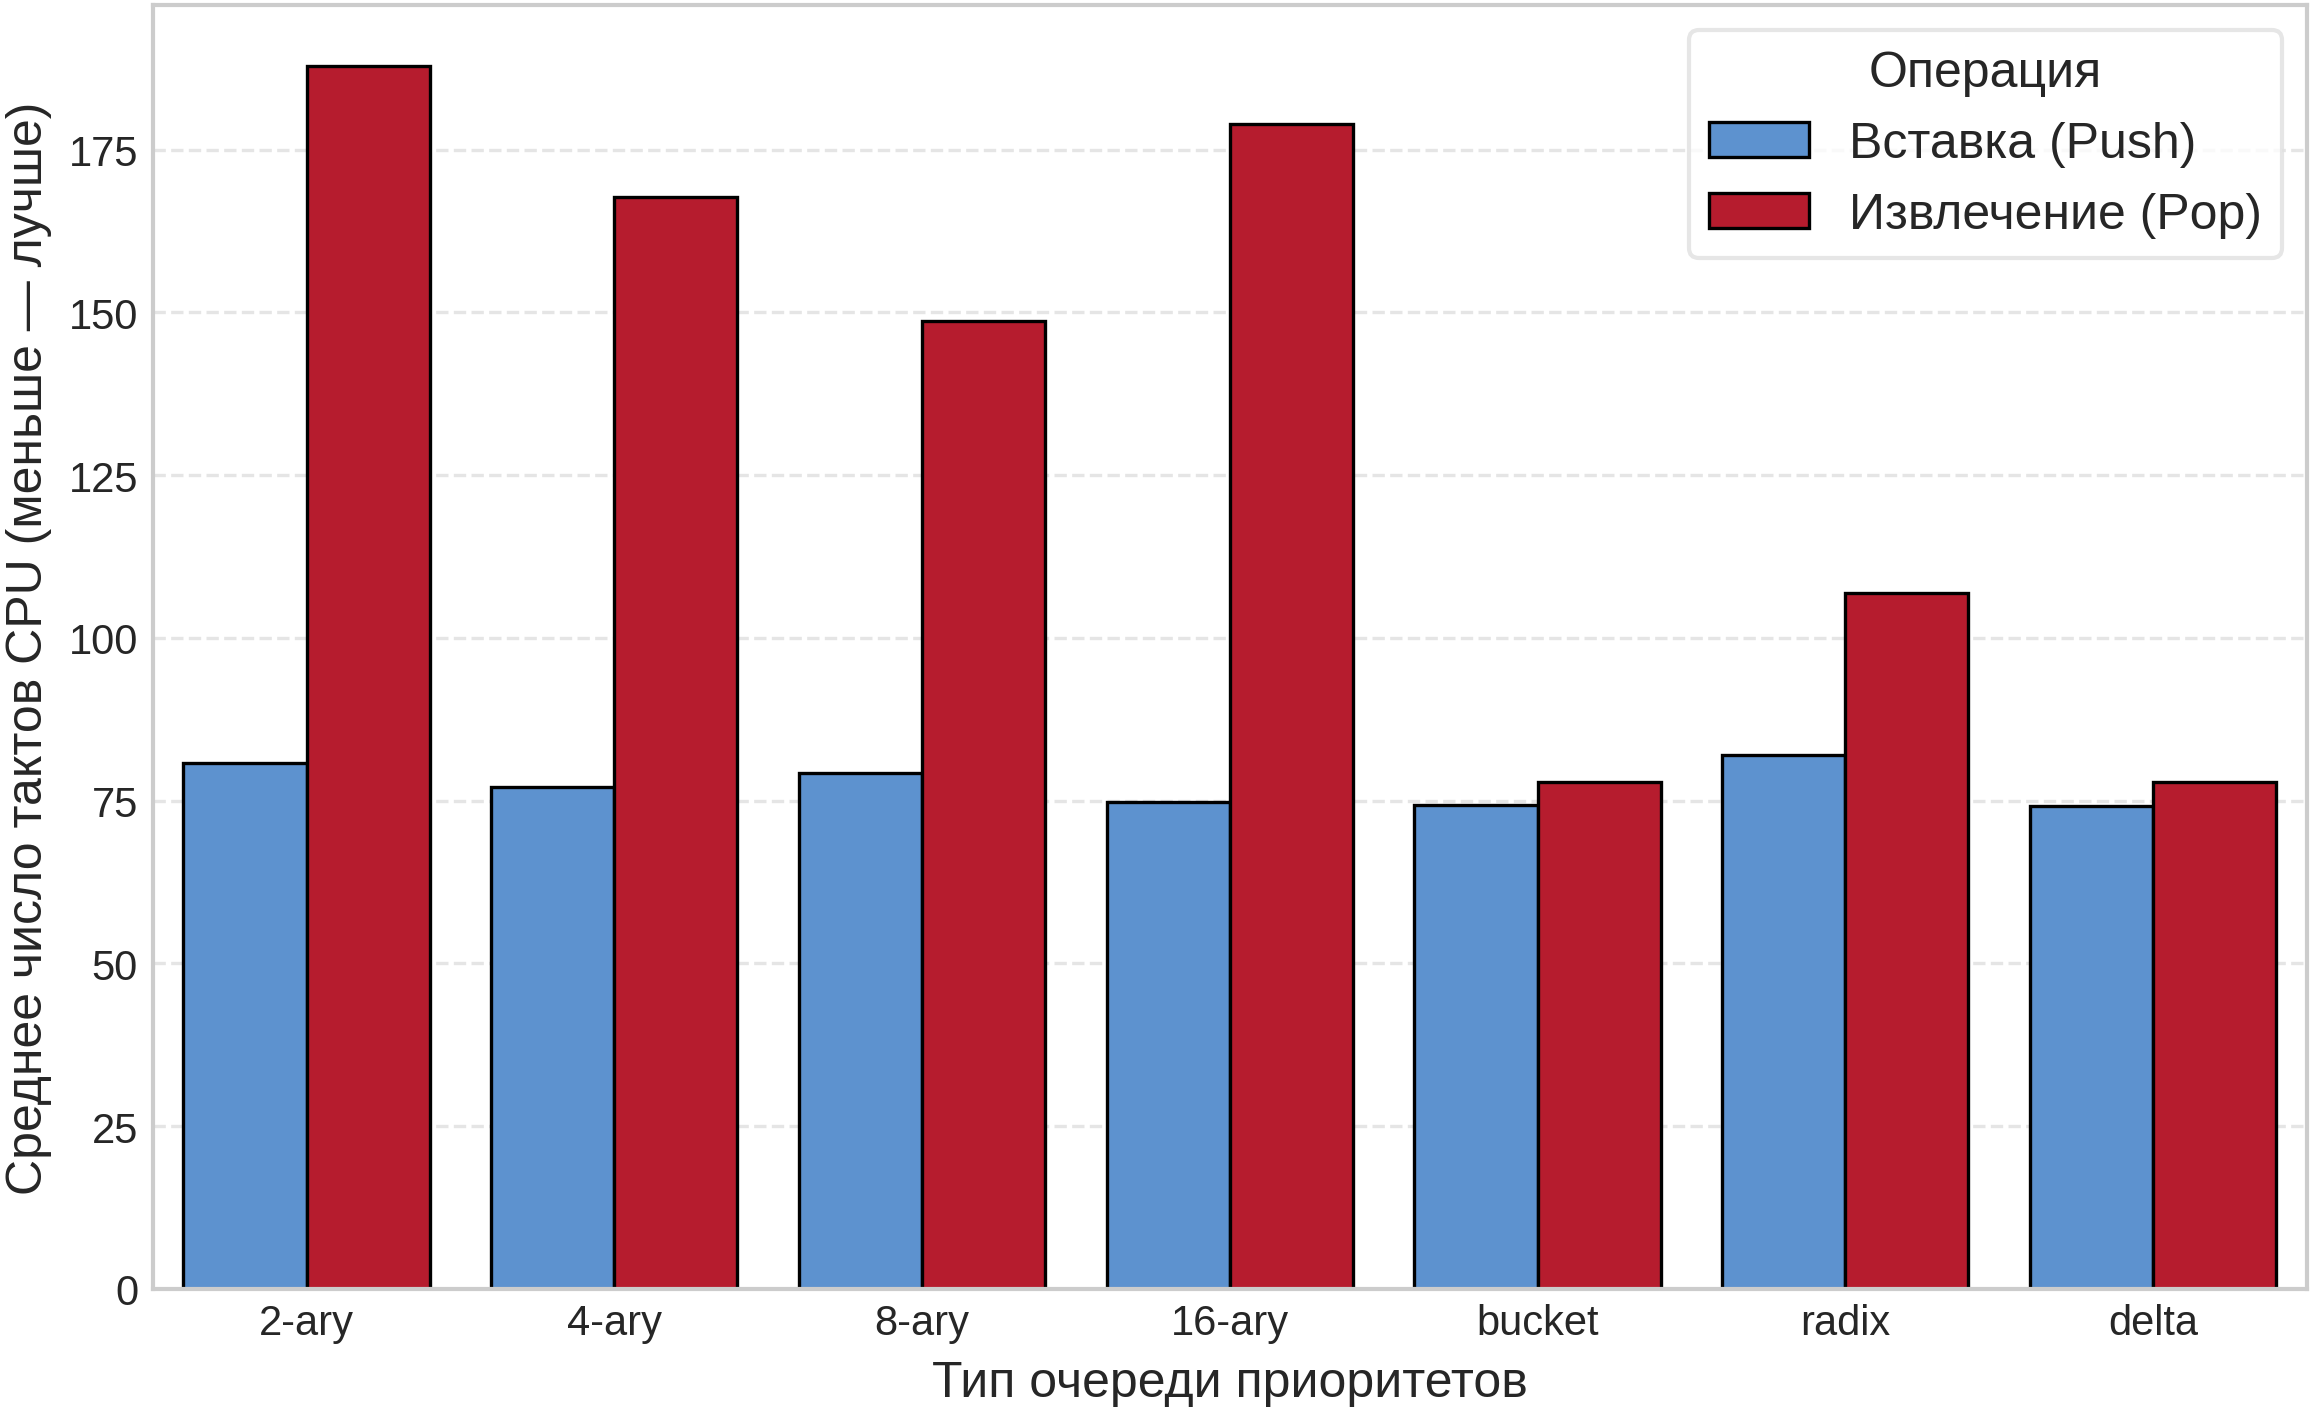
\includegraphics[width=0.85\linewidth,height=0.35\textheight,keepaspectratio]{assets/images/push_pop_cycles_comparison.png}
    \caption{Среднее количество тактов процессора на операции вставки (push) и извлечения (pop) для различных очередей}
    \label{fig:push_pop_cycles_comparison}
\end{figure}

Результаты профилирования показывают, что время вставки для всех очередей сопоставимо ($72$--$92$ такта). Однако операция извлечения сильно различается: для двоичной кучи она выполняется в $2{,}5$--$2{,}7$ раза дольше вставки ($192$--$207$ тактов против $76$--$79$ тактов). Для оптимизированной $8$-арной кучи с совместным кодированием время извлечения снижено до $138$--$154$ тактов, что составляет $1{,}6$--$2{,}0$ раза от времени вставки. Для распределительных очередей время извлечения практически эквивалентно вставке и составляет $77$--$79$ тактов (при $73$--$76$ тактах на вставку).

Измерение динамики накладных расходов в зависимости от длины пути (рис. \ref{fig:queue_overhead_trend}) подтверждает, что операции с очередями составляют значительную часть времени поиска пути: от $40\%$ для распределительных очередей до $65\%$ для древесных куч на сложных маршрутах. Дельта-очередь благодаря константному времени доступа минимизирует эти накладные расходы на всем диапазоне длин маршрутов.

\begin{figure}[htbp]
    \centering
    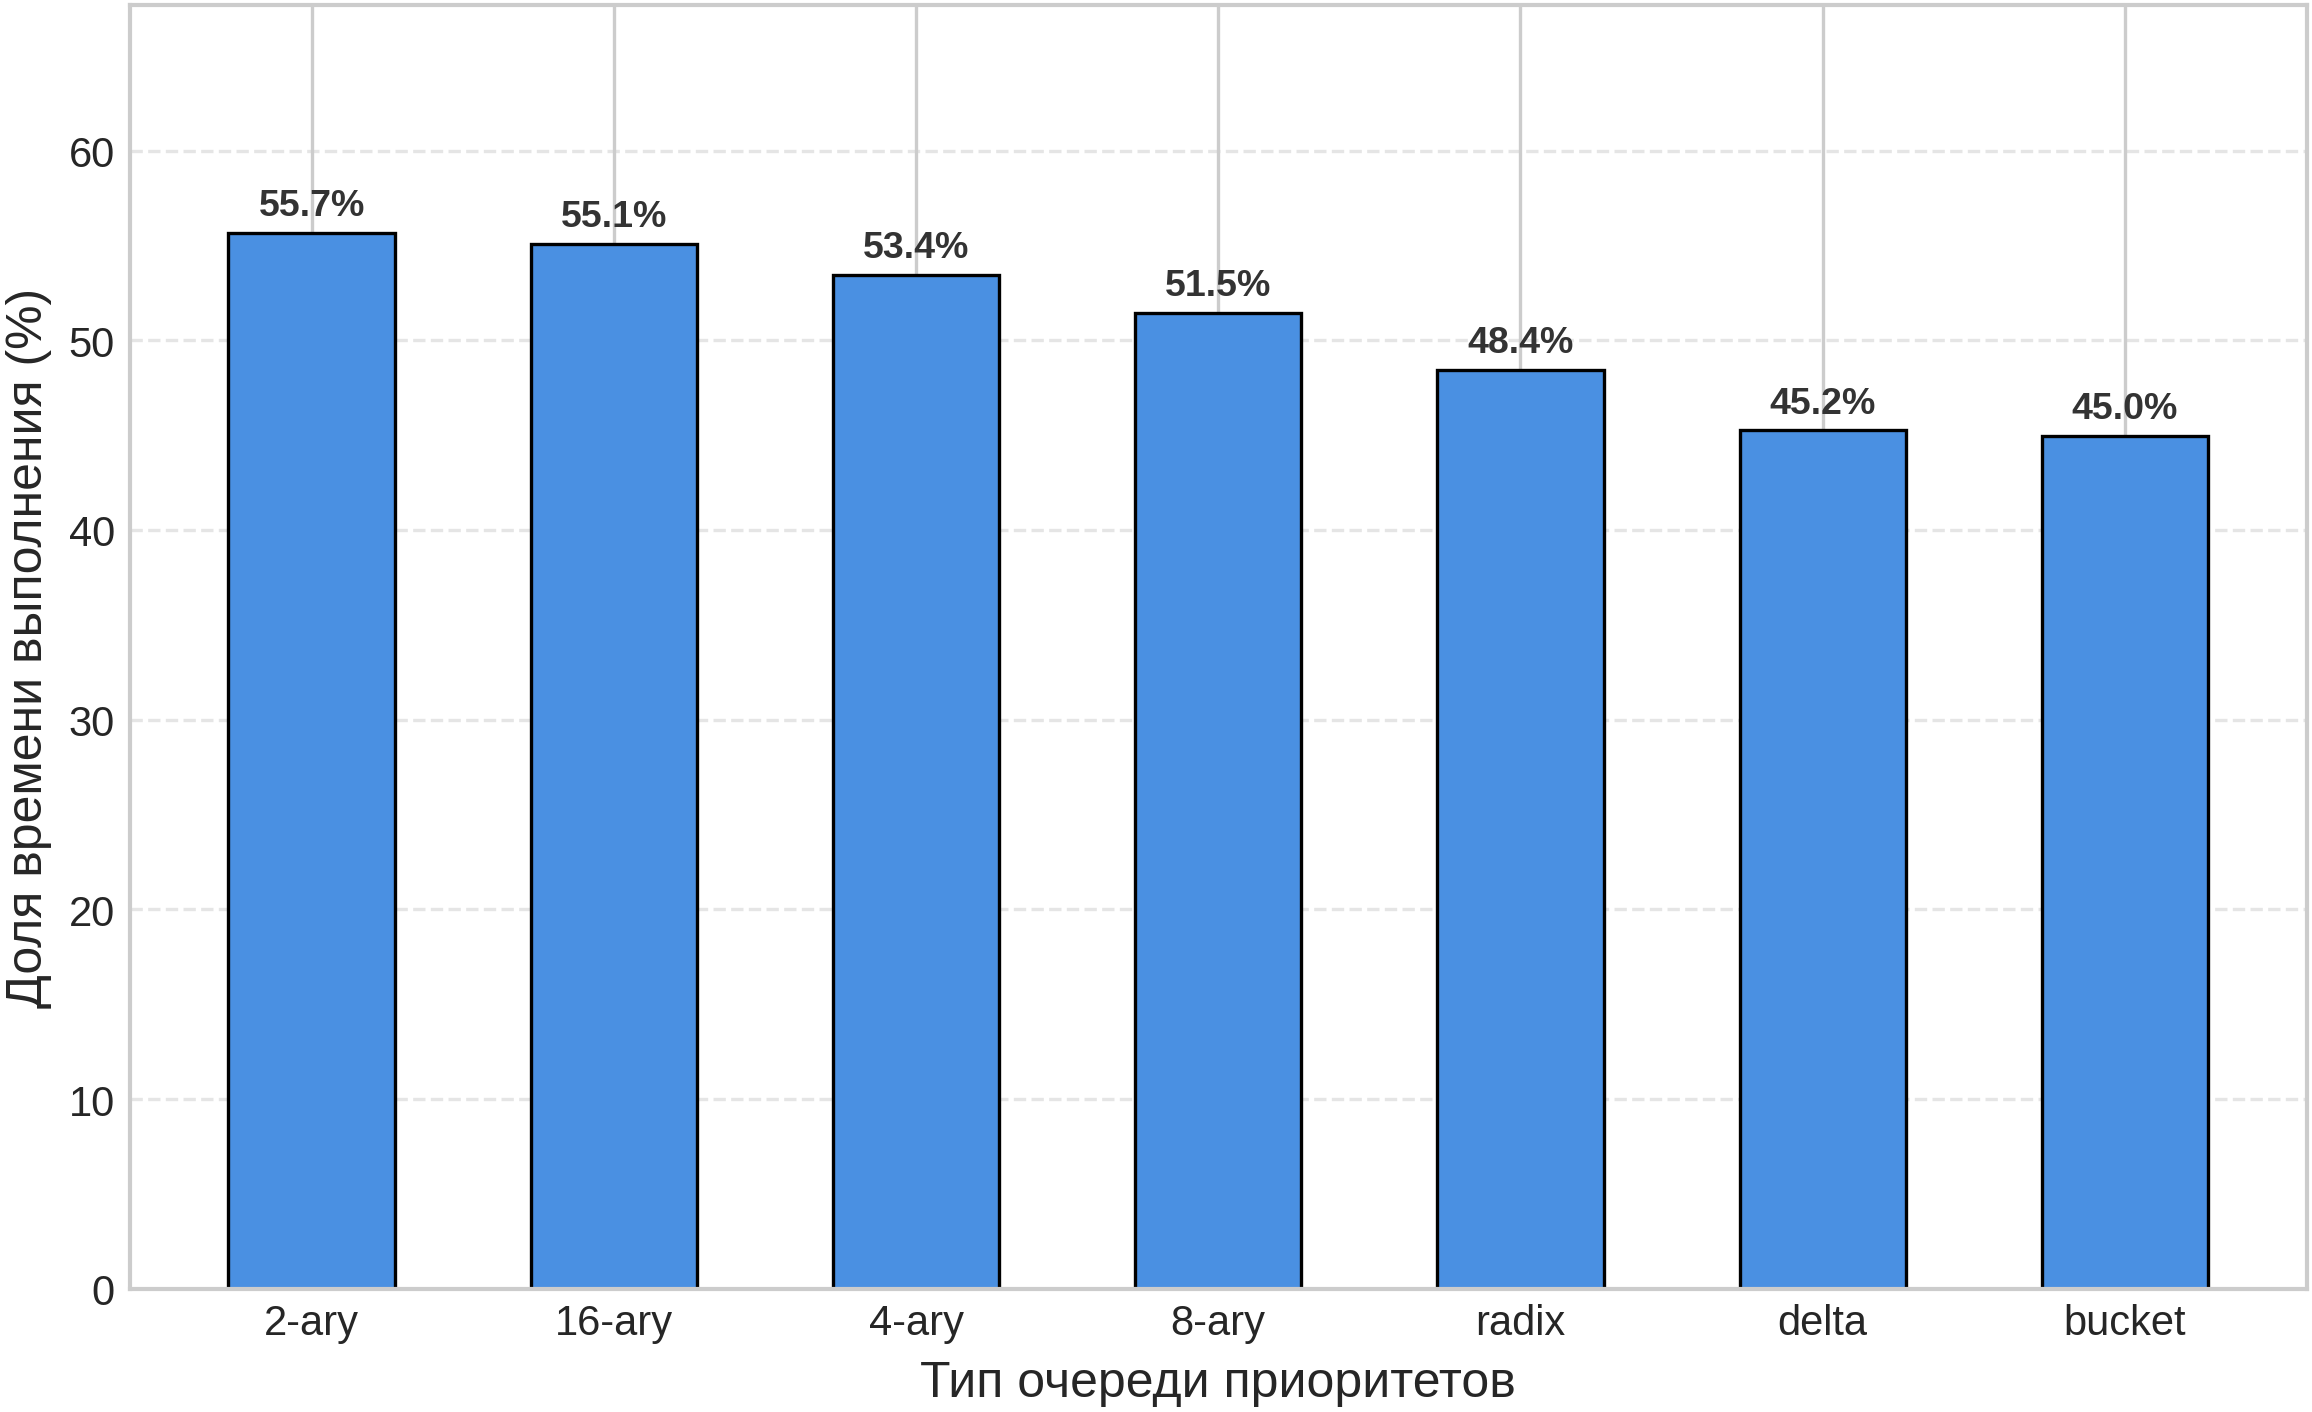
\includegraphics[width=0.85\linewidth,height=0.35\textheight,keepaspectratio]{assets/images/queue_overhead_trend.png}
    \caption{Накладные расходы очередей приоритетов в процентах от общего времени поиска пути с $95\%$-м доверительным интервалом}
    \label{fig:queue_overhead_trend}
\end{figure}

\subsection{Интегральный анализ производительности алгоритмов маршрутизации}
\label{subsec:integral_performance}

По результатам проведенных испытаний построены интегральные графики пропускной способности (выраженной в числе запросов в секунду, $QPS$) в зависимости от сложности маршрута, выраженной в количестве ребер в эталонном кратчайшем пути (рис. \ref{fig:best_combinations_comparison}). Для предотвращения избыточного наложения линий на графике для каждого алгоритма отображены только две лучшие по производительности конфигурации очередей приоритетов. Таким образом, на графике представлены $8$ наиболее эффективных комбинаций: для алгоритмов Дейкстры, двунаправленного поиска и алгоритма $A^*$~-- это дельта-очередь и корзиночная очередь, а для алгоритма $ALT$~-- $4$-арная куча и $8$-арная куча.

\begin{figure}[htbp]
    \centering
    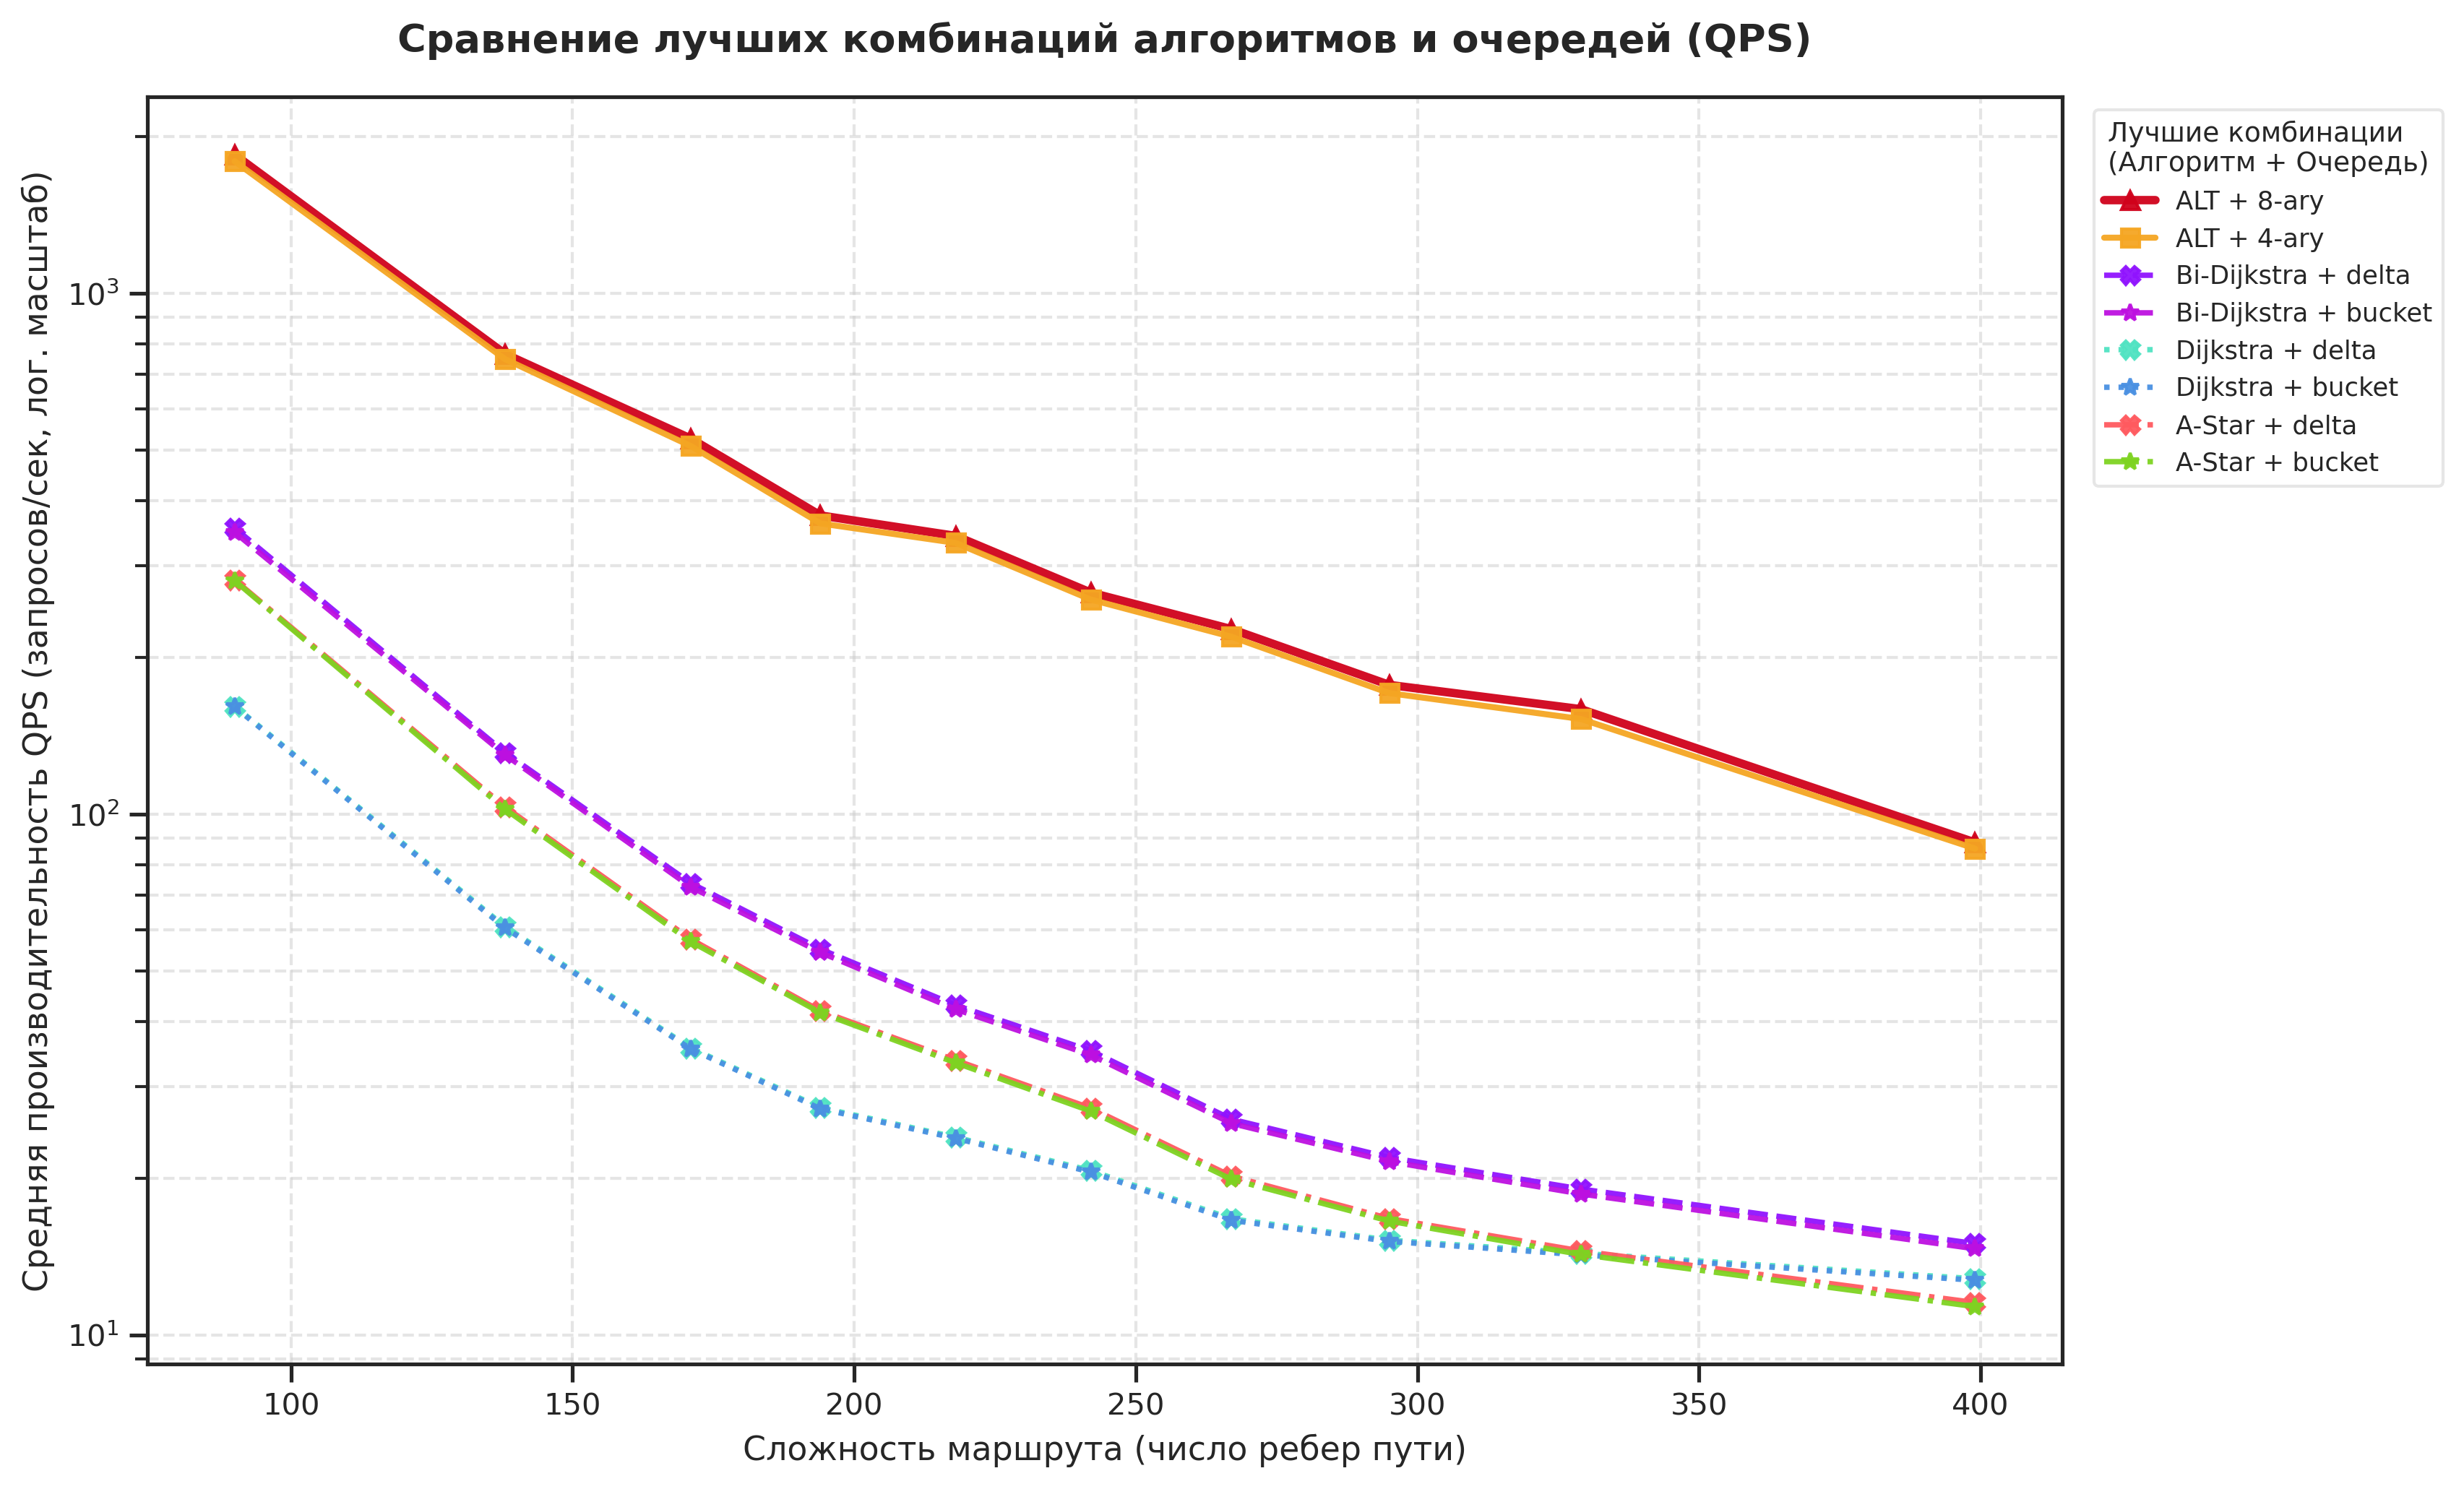
\includegraphics[width=0.85\linewidth,height=0.35\textheight,keepaspectratio]{assets/images/best_combinations_comparison.png}
    \caption{Интегральное сравнение производительности лучших комбинаций алгоритмов поиска пути в зависимости от сложности маршрута}
    \label{fig:best_combinations_comparison}
\end{figure}

Анализ логарифмического графика (рис. \ref{fig:best_combinations_comparison}) позволяет выявить принципиальные различия в поведении алгоритмов при росте длины маршрута. Для традиционных алгоритмов (Дейкстра, двунаправленный поиск, $A^*$) пропускная способность убывает экспоненциально (линейно на логарифмической шкале), что объясняется квадратичным ростом площади поискового пространства. В противовес им, производительность алгоритма $ALT$ имеет немонотонный (скачкообразный) характер с локальными пиками (например, на участках в $250$--$300$ и около $400$ ребер). Это обусловлено тем, что эффективность отсечения вершин в $ALT$ определяется геометрически удачным взаимным расположением заранее вычисленных ориентиров относительно стартовой и целевой точек конкретного маршрута. Тем не менее, во всем диапазоне сложности алгоритм $ALT$ стабильно превосходит остальные подходы минимум на порядок величины.

Примечательно, что классический алгоритм $A^*$ на длинных маршрутах (свыше $300$ ребер) демонстрирует существенное падение производительности, сближаясь с показателями базового алгоритма Дейкстры. Это свидетельствует о слабой направляющей способности стандартной эвристики евклидового расстояния в условиях сложной топологии городской сети. Второе место по уровню пропускной способности уверенно удерживает двунаправленный алгоритм Дейкстры. Однако, несмотря на высокие показатели, двунаправленный поиск неприменим в разработанном вычислительном ядре динамического регулирования из-за отсутствия темпорального детерминизма обратной волны при предиктивном резервировании емкостей дорожной сети (см. подраздел \ref{subsec:bidirectional_limitations}).

Особое внимание на графике \ref{fig:best_combinations_comparison} стоит уделить дельта-очереди, которая в алгоритмах Дейкстры, $A^*$ и двунаправленного поиска показывает топовые результаты наравне с корзиночной очередью за счет алгоритмической сложности $O(1)$.

Однако детальное сравнение очередей исключительно для алгоритма $ALT$ (рис. \ref{fig:alt_qps_comparison}) наглядно демонстрирует, что распределительные очереди (дельта и корзины) стабильно проигрывают классическим многоарным кучам на всем диапазоне сложности маршрута. Хуже всего справляется поразрядная куча (radix). Радикальное сужение области поиска в $ALT$ приводит к тому, что древовидные структуры работают исключительно в быстрой кэш-памяти без глубоких логарифмических задержек. В этих условиях накладные расходы на инициализацию и обход пустых ведер в распределительных очередях становятся избыточными. 

\begin{figure}[htbp]
    \centering
    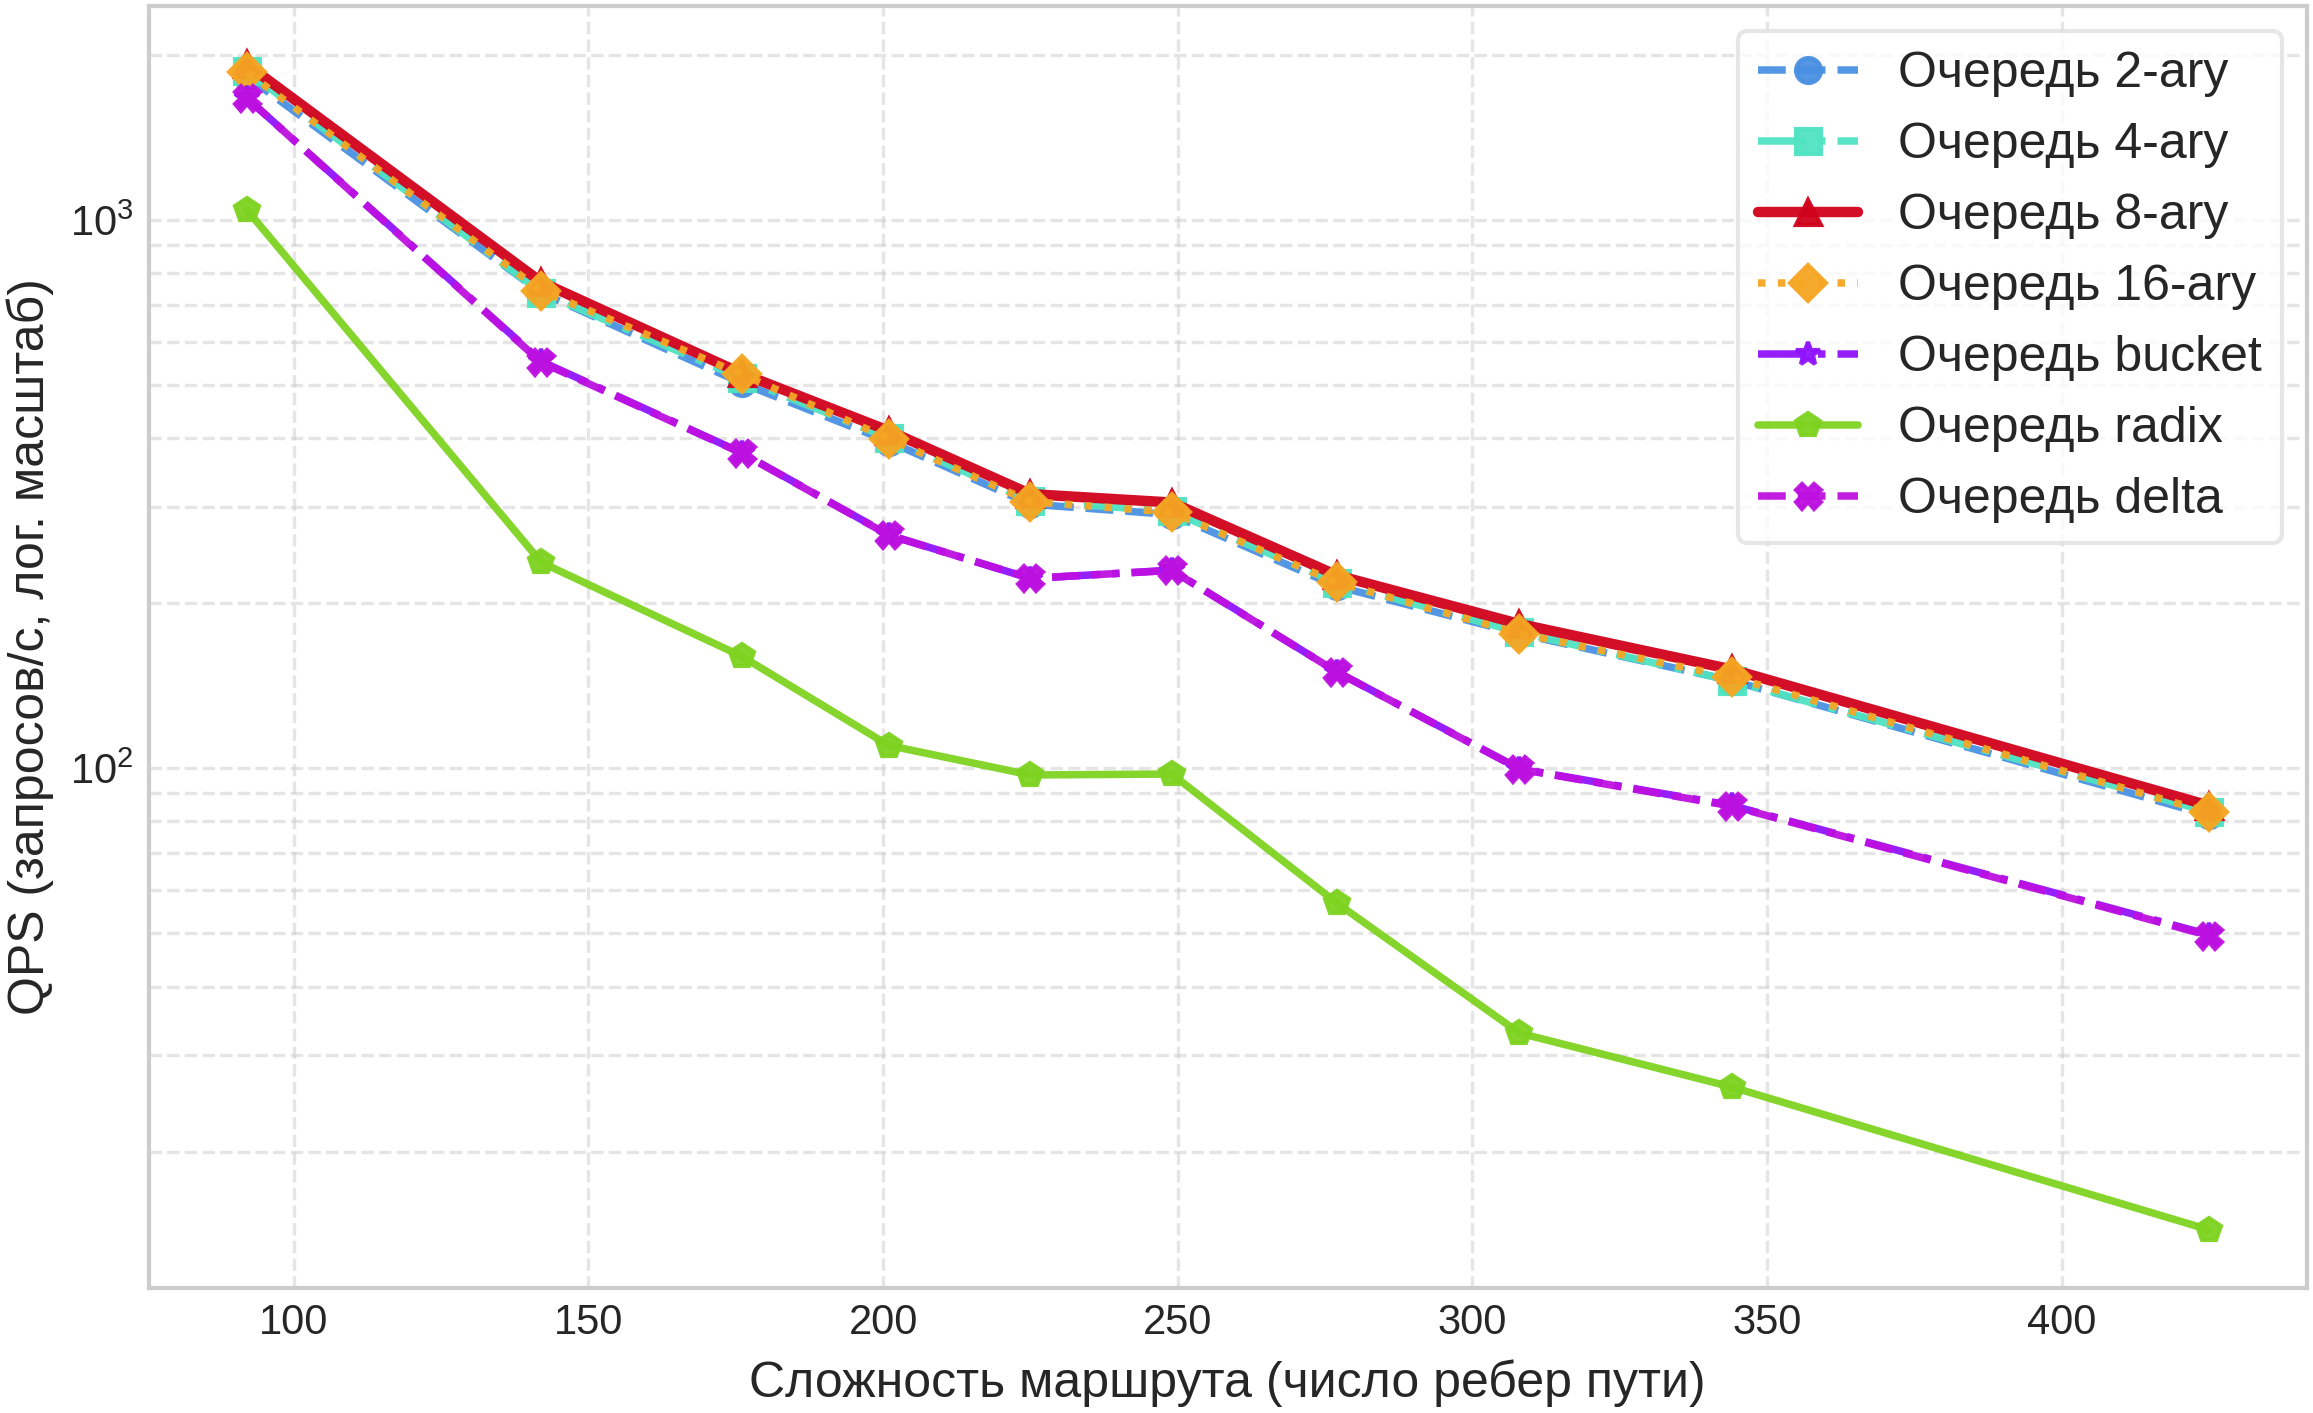
\includegraphics[width=0.85\linewidth,height=0.35\textheight,keepaspectratio]{assets/images/alt_qps_comparison.png}
    \caption{Производительность поиска пути ALT в зависимости от длины маршрута для различных очередей}
    \label{fig:alt_qps_comparison}
\end{figure}

На графике видно, что благодаря совместному кодированию ключа и индекса $8$-арная куча превосходит остальные многоарные структуры, демонстрируя наивысшую производительность во всем диапазоне сложности и достигая $245$ запросов в секунду (QPS) на алгоритме $ALT$. Такое решение продиктовано строгим соответствием параметров структуры аппаратной архитектуре: $8$ дочерних элементов по $32$ бита каждый в сумме составляют ровно $256$ бит. Это позволяет на $100\%$ утилизировать ширину одного векторного регистра AVX2 за одну инструкцию — без простоя вычислительных блоков (как в случае с $4$-арной кучей) и без разбиения поиска минимального потомка на несколько векторных операций (как в $16$-арной куче). Таким образом, $8$-арная куча представляет собой архитектурно наиболее эффективное решение для ядра маршрутизации, максимизирующее пропускную способность.

\subsection{Исследование многопоточной масштабируемости и системной оптимизации привязки потоков}

Для исследования масштабируемости программа измеряет пропускную способность на шестиядерном процессоре при изменении количества рабочих потоков для лучшей конфигурации алгоритма $ALT$ с $8$-арной кучей. Тестирование проходило в двух режимах: со стандартным распределением потоков операционной системой Arch Linux и с жесткой аппаратной привязкой потоков к физическим ядрам процессора. Рисунок \ref{fig:multithreading_scalability} показывает результаты сравнения.

\begin{figure}[htbp]
    \centering
    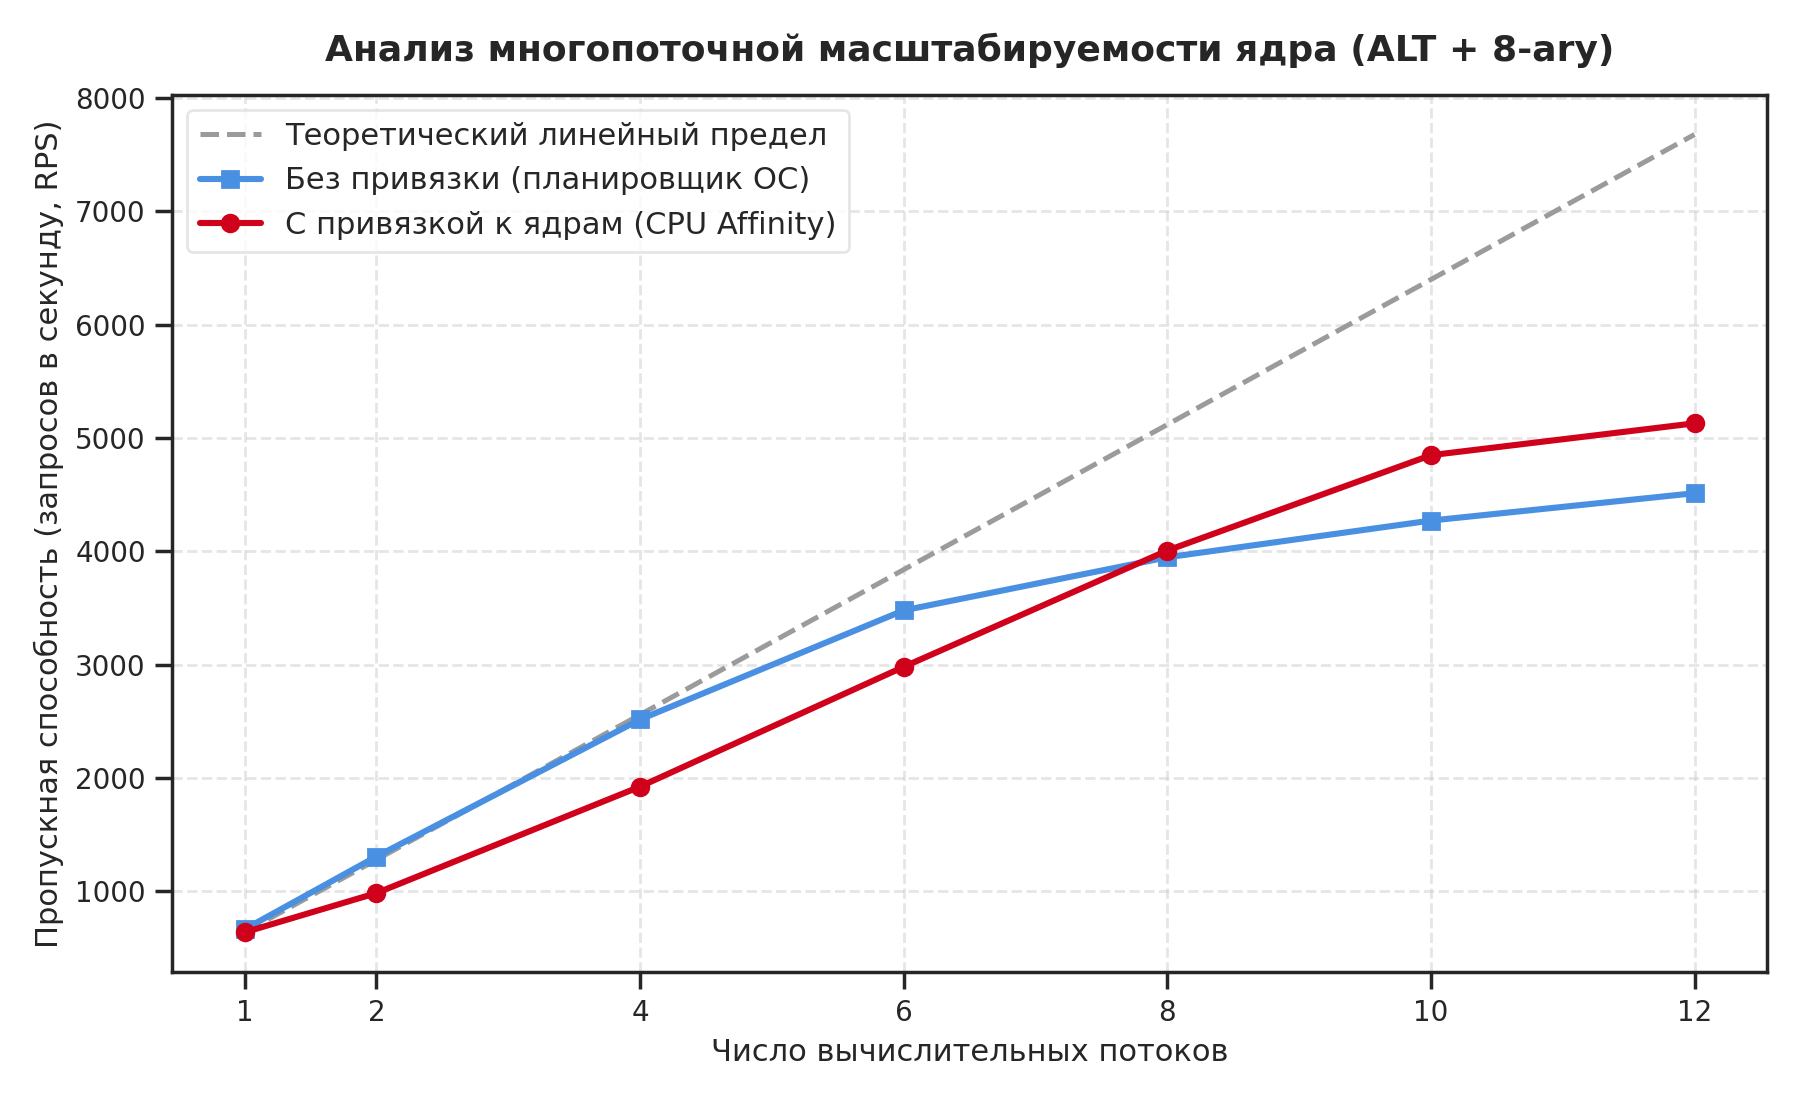
\includegraphics[width=0.85\linewidth,height=0.35\textheight,keepaspectratio]{assets/images/multithreading_scalability.png}
    \caption{Сравнение теоретического предела и фактической пропускной способности многопоточного ядра на базе алгоритма $ALT$ и $8$-арной кучи}
    \label{fig:multithreading_scalability}
\end{figure}

Анализ масштабируемости выявляет четкую границу применимости жесткой привязки потоков к ядрам. До $8$ потоков лидирует стандартный планировщик ОС: он динамически разносит потоки по свободным физическим ядрам ЦП, обеспечивая монопольный доступ к АЛУ и кэшам L1/L2. Жесткая привязка на этом этапе искусственно создает конкуренцию за ресурсы внутри физического ядра. Однако при плотной загрузке свыше $8$ потоков планировщик ОС начинает слишком часто мигрировать потоки, вызывая массовые промахи кэша. Здесь жесткая привязка фиксирует потоки и стабилизирует ядро: на предельных $12$ потоках она обеспечивает $5130$ QPS, обгоняя планировщик на $13{,}6\%$.

Таким образом, масштаб проведенного экспериментального исследования ($28$ комбинаций алгоритмов и очередей, протестированных на $500$ разнородных пространственных задачах~-- суммарно более $14000$ полных циклов трассировки на реальном субграфе Москвы) обеспечивает репрезентативность выборки. Дополнительное варьирование параметра эвристики $w$ или отключение эвристического веса является избыточным, так как результаты согласуются с теоремой о субоптимальности, в то время как выбранный режим $w = 1{,}15$ доказал свою сбалансированность для геоинформационных систем реального времени.

\section{Экспериментальное исследование асинхронной симуляции и динамического регулирования}

\subsection{Экспериментальное исследование динамики распределения транспортных потоков}
Динамика асинхронного управляющего контура исследована на субграфе дорожной сети Москвы при нагрузке в $200~000$ активных транспортных средств с масштабным фактором агентов $ASF = 1{,}0$ (один агент соответствует одному автомобилю).

Выбранный объем нагрузки в $200~000$ агентов аппроксимирует интенсивность движения в межпиковые периоды (что сопоставимо с емкостью дорожной сети Москвы в периоды спада маятниковой миграции при условном максимуме до $400~000$ одновременно движущихся автомобилей). Использование стохастического распределения пунктов отправления и назначения (OD-матрицы) позволяет абстрагироваться от направленных маятниковых потоков и воспроизвести изотропную фоновую загрузку городской сети. Для оптимизации вычислительных затрат применяется масштабный коэффициент агентов $ASF$ (раздел~\ref{sec:agent-space}). Однако агрегирование транспортных единиц ($ASF > 1{,}0$) приводит к геометрическому искажению емкости узких мест, особенно на коротких ребрах графа, что маскирует пространственно-временное распространение обратных заторов (spillback). Несмотря на то, что расчет очередей и гидродинамического давления потока локализован в агентном пространстве, данное искажение снижает адекватность моделирования. Ввиду отсутствия базовой динамической сходимости в текущих сценариях, дальнейшее масштабирование числа агентов или варьирование коэффициента $ASF$ признано нецелесообразным до решения фундаментальной задачи стабилизации динамического локального маршрутизирования.

Эксперимент показал расходимость транспортной системы из-за отсутствия глобального координатора и запаздывания обратной связи. Наличие временной задержки в контуре управления вызывает маятниковую неустойчивость. Локальные заторы накапливаются, что приводит к росту общего индекса задержки сети ($TTI$). Вместо стабилизации и достижения динамического равновесия Уордропа система демонстрирует переходный процесс с выраженной пространственно-временной расходимостью. Подробный анализ этого процесса приведен далее.

\subsection{Анализ фундаментальных ограничений дискретной мезоскопической модели}

Для детального исследования физических эффектов проанализирована динамика симуляции с включенным динамическим регулированием.

Индекс задержки $TTI$ (рис. \ref{fig:sim_tti}) разделяется на несколько характерных фаз. На графике сглаженный тренд (скользящее среднее по окну $600$~с) отражает глобальные макроскопические изменения задержек в сети, в то время как затененная область показывает диапазон локального среднеквадратического отклонения флуктуаций ($\pm\sigma$). Индекс задержки имеет начальный локальный максимум около отметки $4000$~с ($TTI \approx 3{,}4$), после чего снижается до локального минимума на $12~000$~с ($TTI \approx 2{,}8$). Начиная с $12~000$~с, средний индекс $TTI$ возрастает вплоть до отметки $10{,}1$ к концу симуляции. Рост ширины зоны дисперсии указывает на нарастание колебательного процесса: агенты реагируют на динамические веса ребер и перестраиваются на одни и те же альтернативные маршруты, вызывая их циклическую перегрузку.

При этом график накопленных завершенных поездок (рис. \ref{fig:sim_completed_trips}) демонстрирует рост на протяжении всей симуляции, достигая $1{,}35$~млн автомобилей к концу теста. Трафик поглощает стартовый пиковый объем, однако система не стабилизируется. Рост числа завершенных поездок подтверждает сохранение работоспособности сети при увеличении времени движения по маршрутам.

\begin{figure}[htbp]
    \centering
    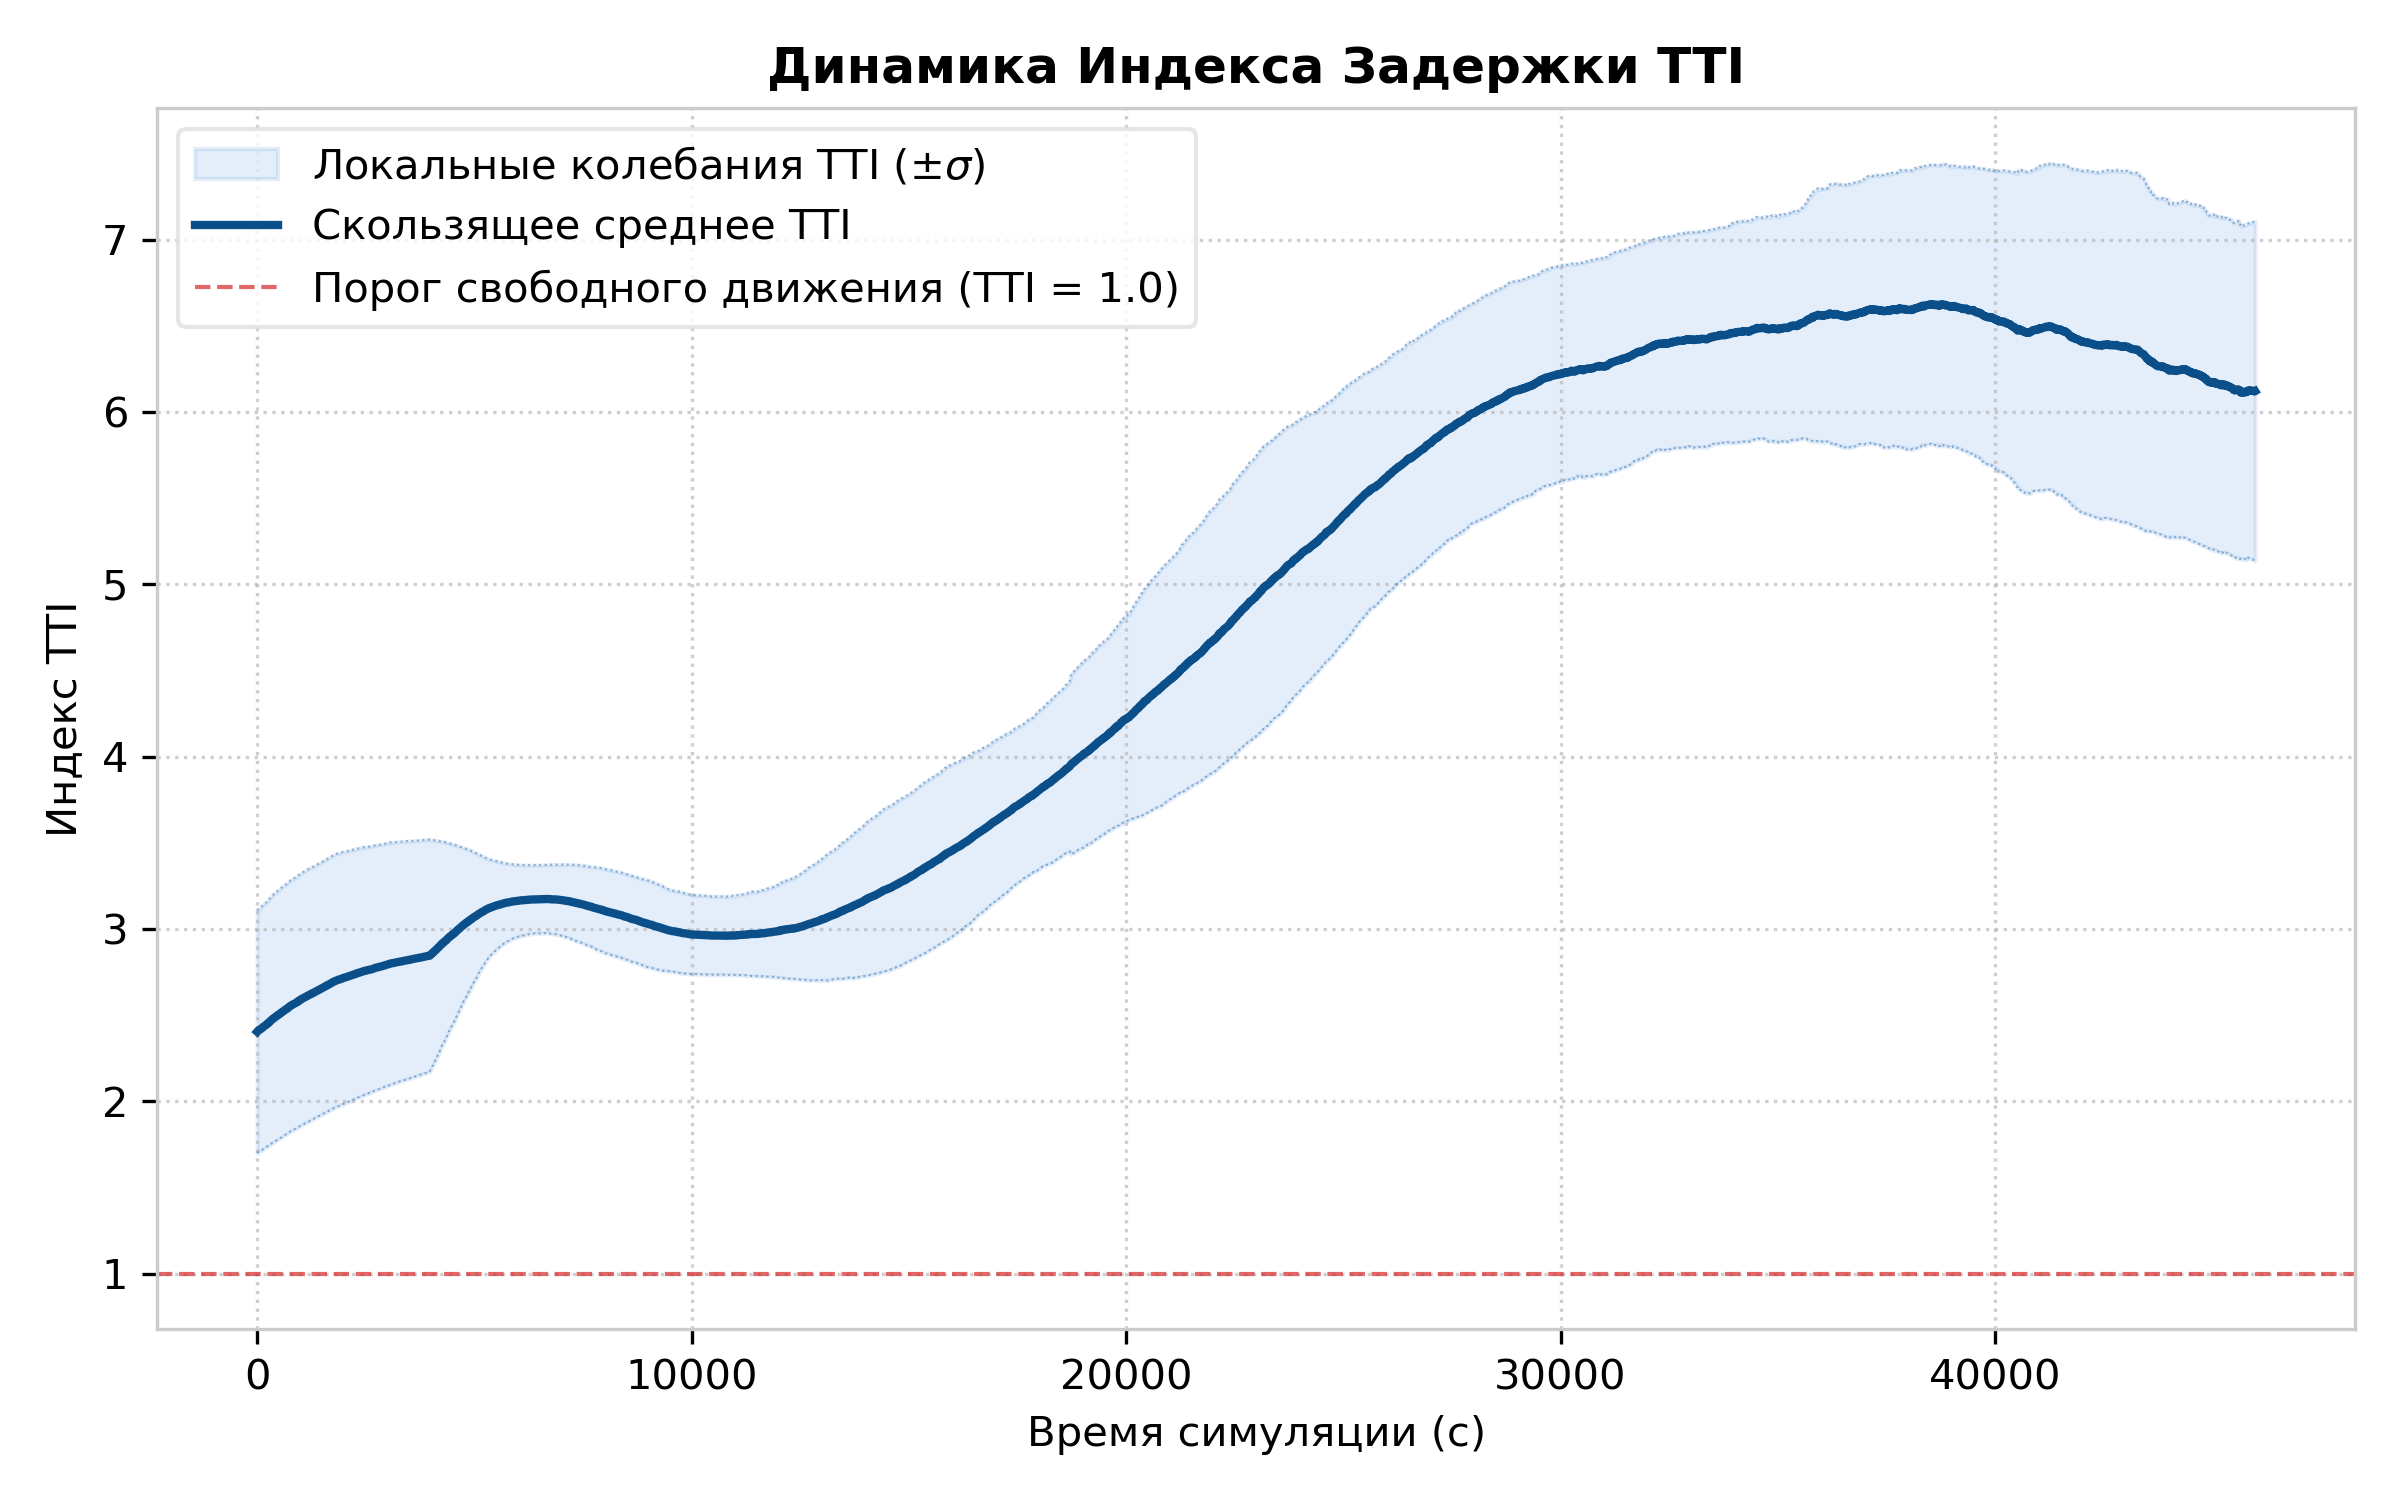
\includegraphics[width=0.85\linewidth,keepaspectratio]{assets/images/fig_tti.png}
    \caption{Динамика Индекса Задержки $TTI$ в ходе симуляции}
    \label{fig:sim_tti}
\end{figure}

\begin{figure}[htbp]
    \centering
    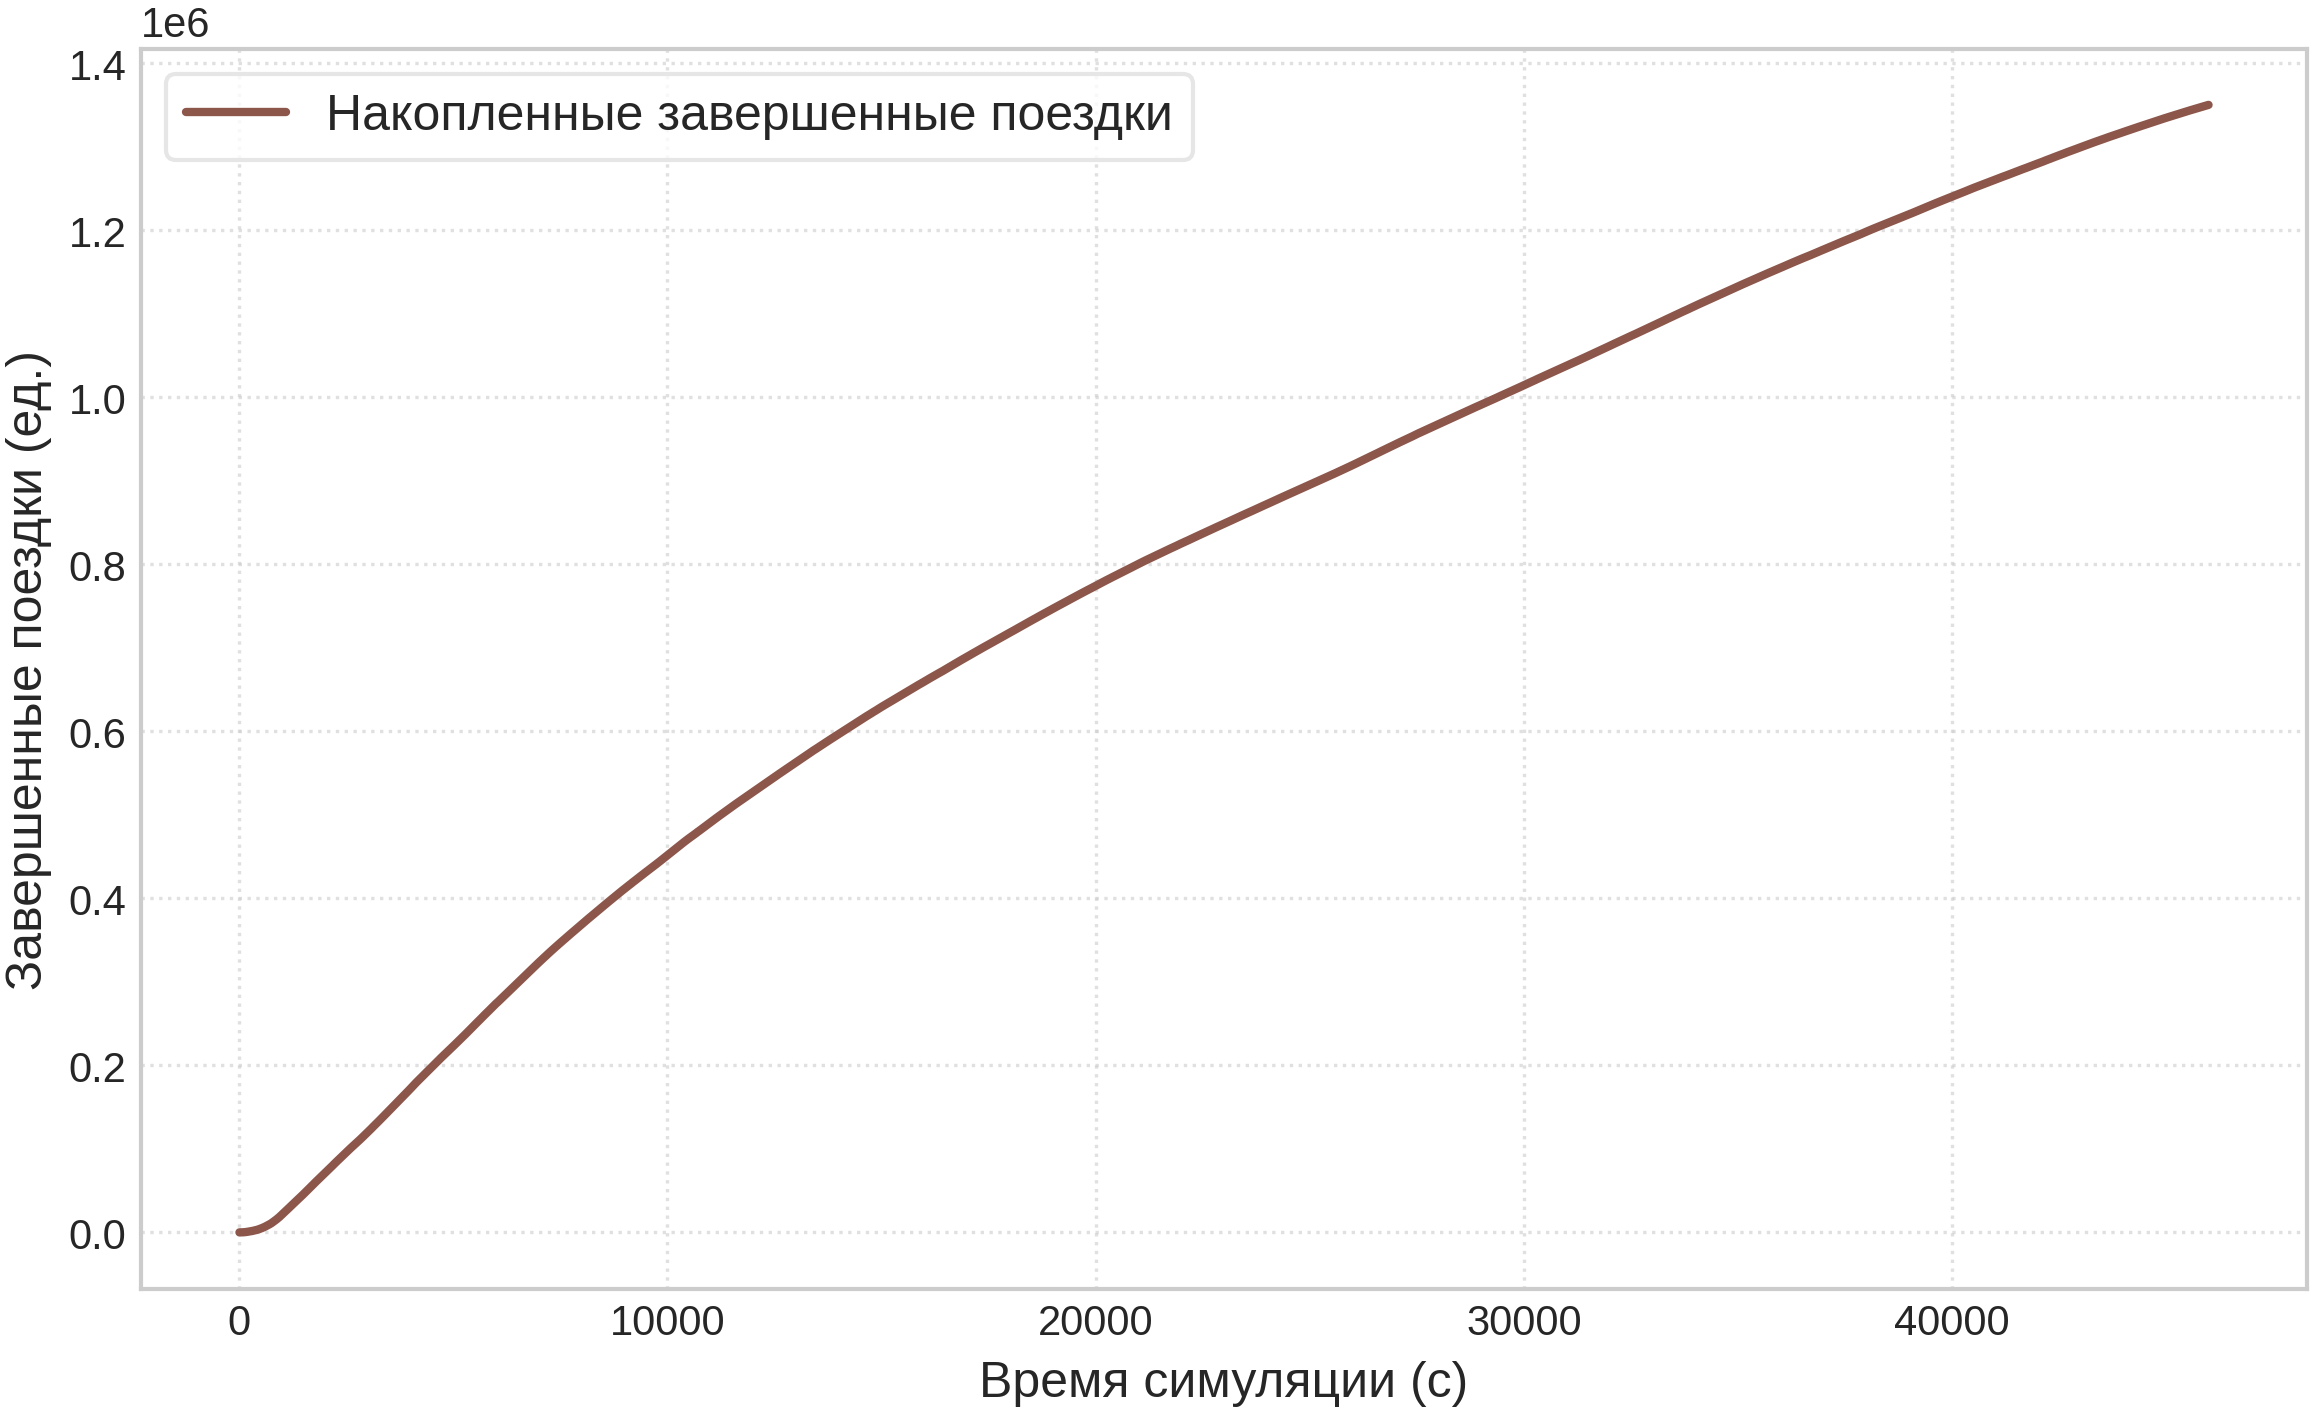
\includegraphics[width=0.85\linewidth,keepaspectratio]{assets/images/fig_completed_trips.png}
    \caption{Интегральная пропускная способность (накопленные завершенные поездки)}
    \label{fig:sim_completed_trips}
\end{figure}

Классификация состояний ребер по плотности и соответствующим им скоростным диапазонам приведена в табл. \ref{tab:traffic_zones}.

\begin{table}[htbp]
    \caption{Классификация состояний ребер дорожного графа по плотности потока}
    \label{tab:traffic_zones}
    \centering
    \begin{tabular}{|l|c|c|p{5.5cm}|}
        \hline
        Цветовая зона & Математическое условие & Скорость $v_{actual}$ & Состояние потока \\ \hline
        Зеленая & $N_{cars} < C_{vis} + 0{,}3(C_{jam} - C_{vis})$ & $> 0{,}97 V_{free}$ & Свободный поток, минимальная задержка \\ \hline
        Желтая & $C_{vis} + 0{,}3(C_{jam} - C_{vis}) \le N_{cars} < C_{jam}$ & $(0{,}83; 0{,}97] V_{free}$ & Плотный поток, возникновение взаимных помех \\ \hline
        Красная & $C_{jam} \le N_{cars} < 2 C_{jam}$ & $[V_{free}/11; 0{,}83] V_{free}$ & Перегрузка, задержка до $10 T_{free}$, скорость падает до $V_{free}/11$ ($5{,}45$~км/ч при лимите $60$~км/ч, $8{,}18$~км/ч при $90$~км/ч) \\ \hline
        Черная & $N_{cars} \ge 2 C_{jam}$ & $0$ & Блокировка ребра ($v_{actual} = 0$), рост обратного затора \\ \hline
    \end{tabular}
\end{table}

Динамика количества свободных ребер (рис. \ref{fig:sim_green_zones}) фиксирует пространственное стягивание потоков. После начального спада количество зеленых ребер кратковременно восстанавливается до $62$~тыс. на $7000$~с, после чего снижается до $27$~тыс. к концу симуляции. В этот же период число перегруженных сегментов в красной и черной зонах суммарно увеличивается с $1210$ до $3578$ (рис. \ref{fig:sim_red_yellow_zones}). Это доказывает, что транспортные средства концентрируются на ограниченном количестве альтернативных маршрутов, полностью исчерпывая их емкость, в то время как остальная часть дорожной сети остается неиспользуемой.

\begin{figure}[htbp]
    \centering
    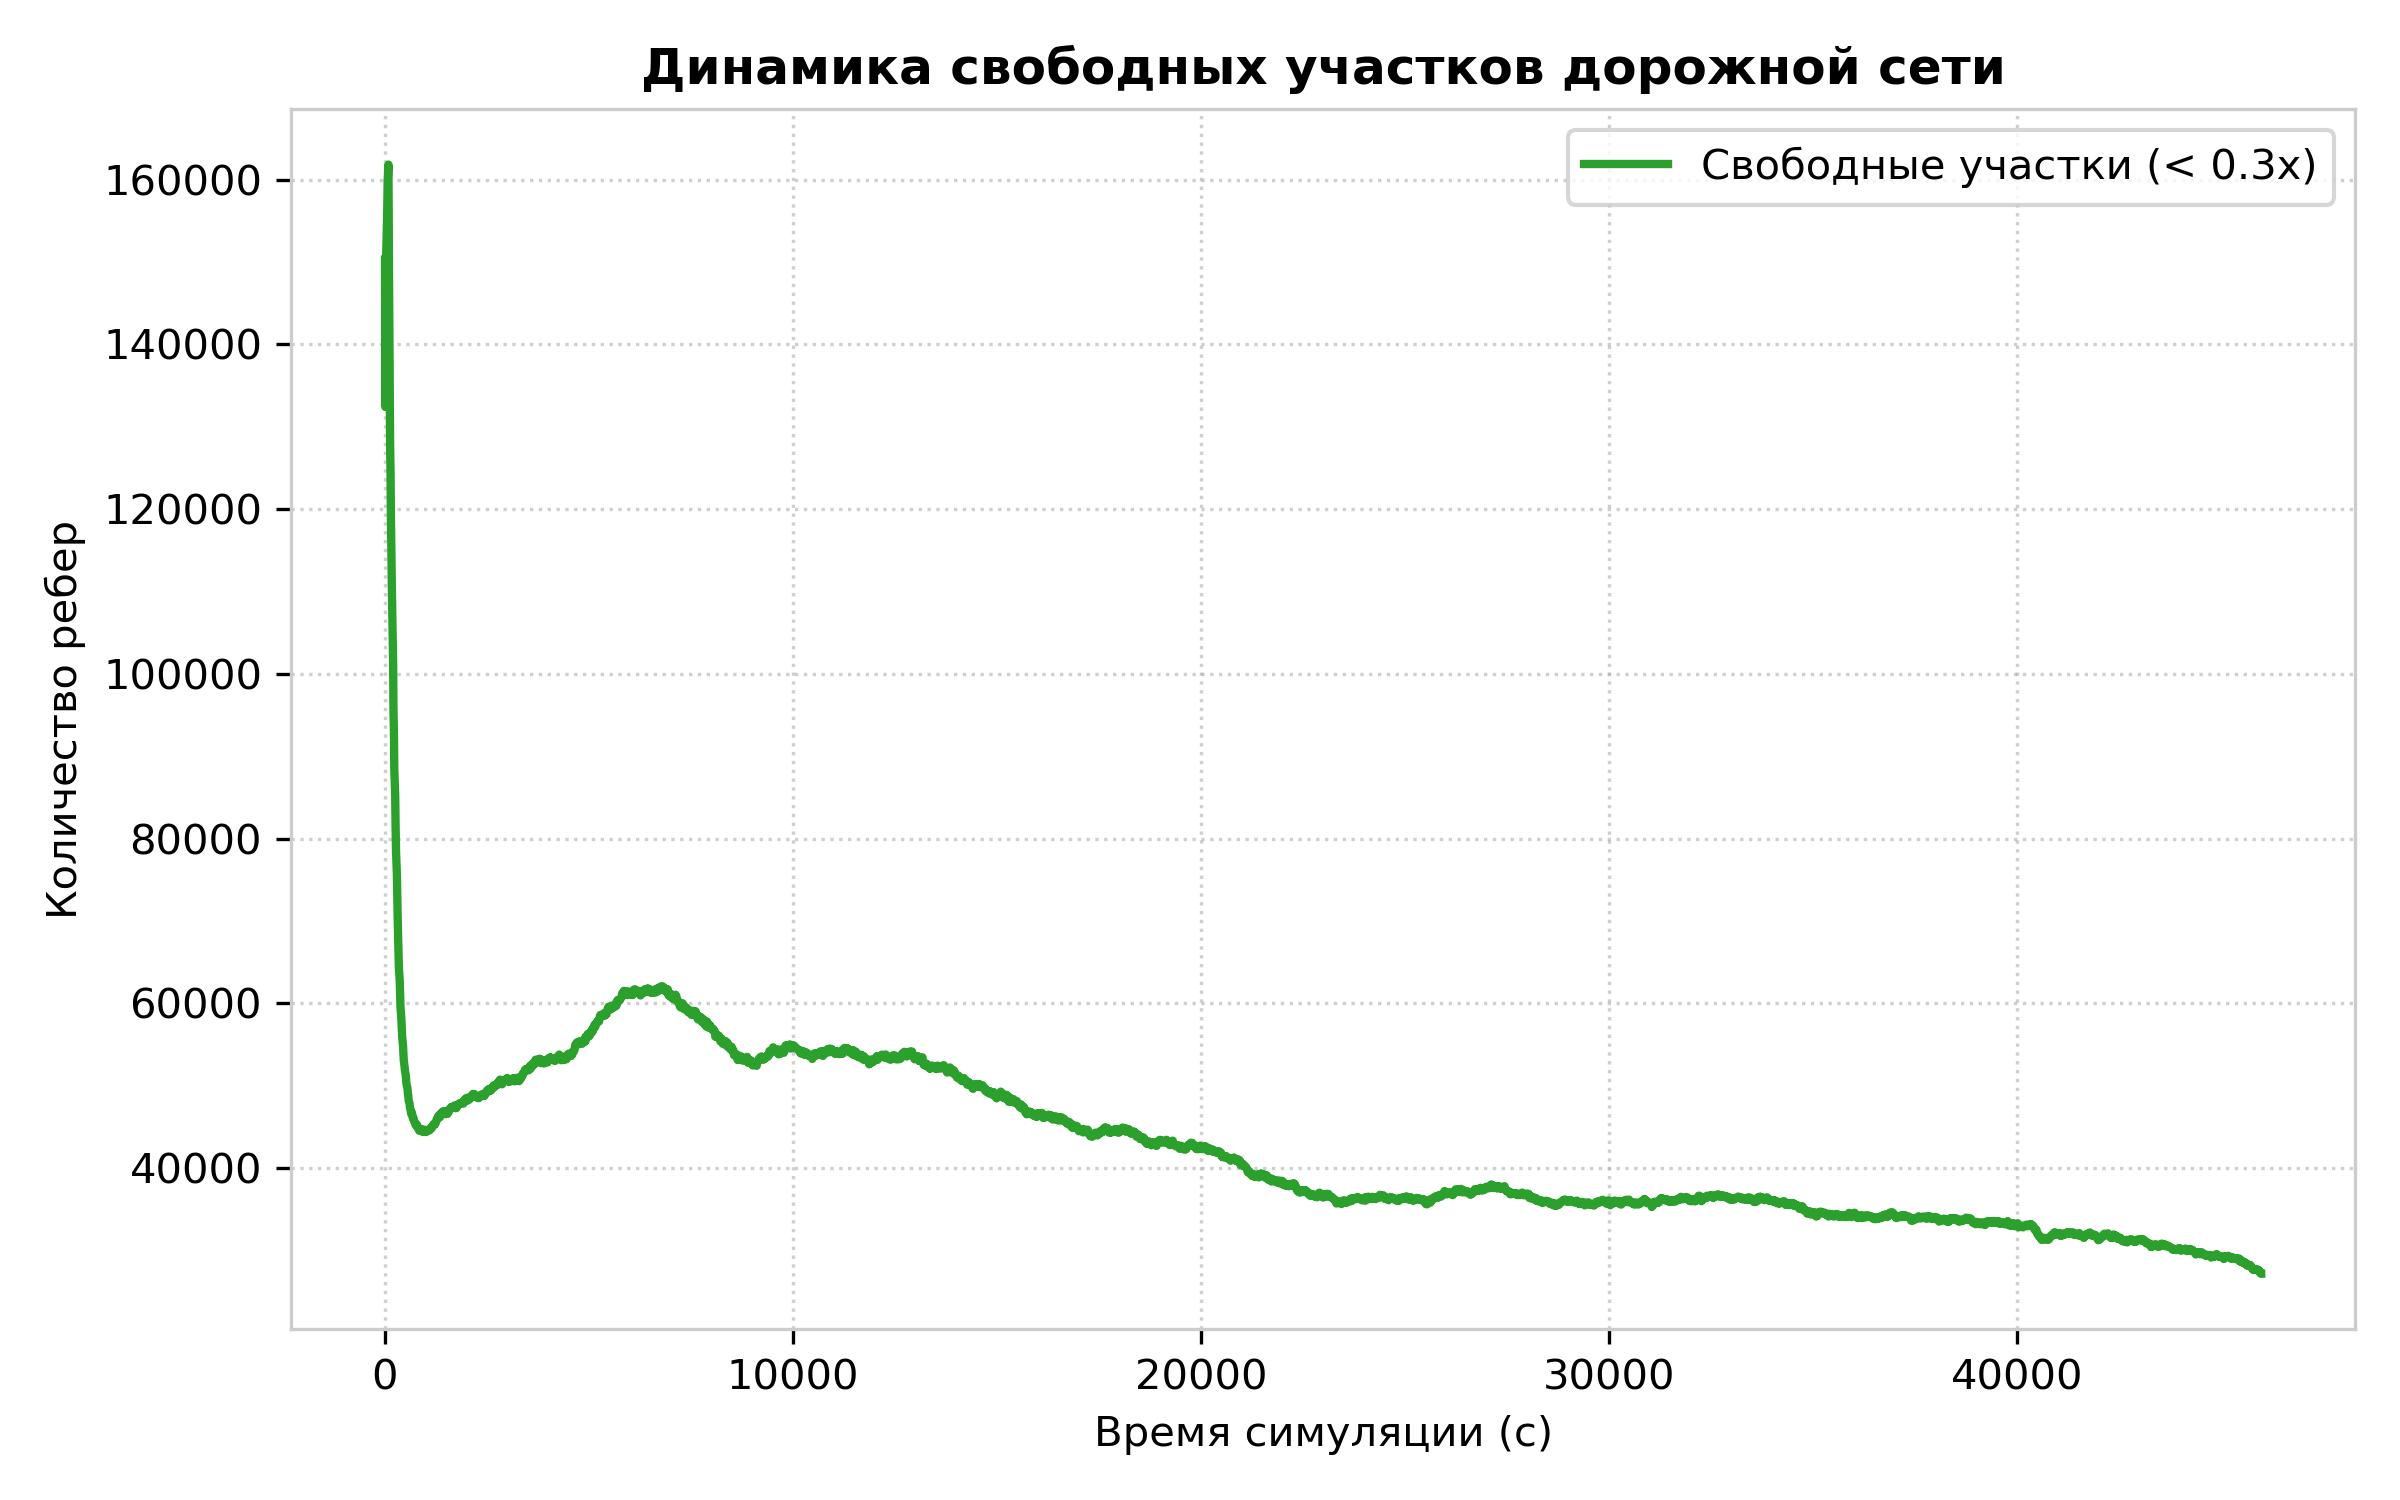
\includegraphics[width=0.85\linewidth,keepaspectratio]{assets/images/fig_green_zones.png}
    \caption{Динамика количества свободных участков дорожной сети}
    \label{fig:sim_green_zones}
\end{figure}

\begin{figure}[htbp]
    \centering
    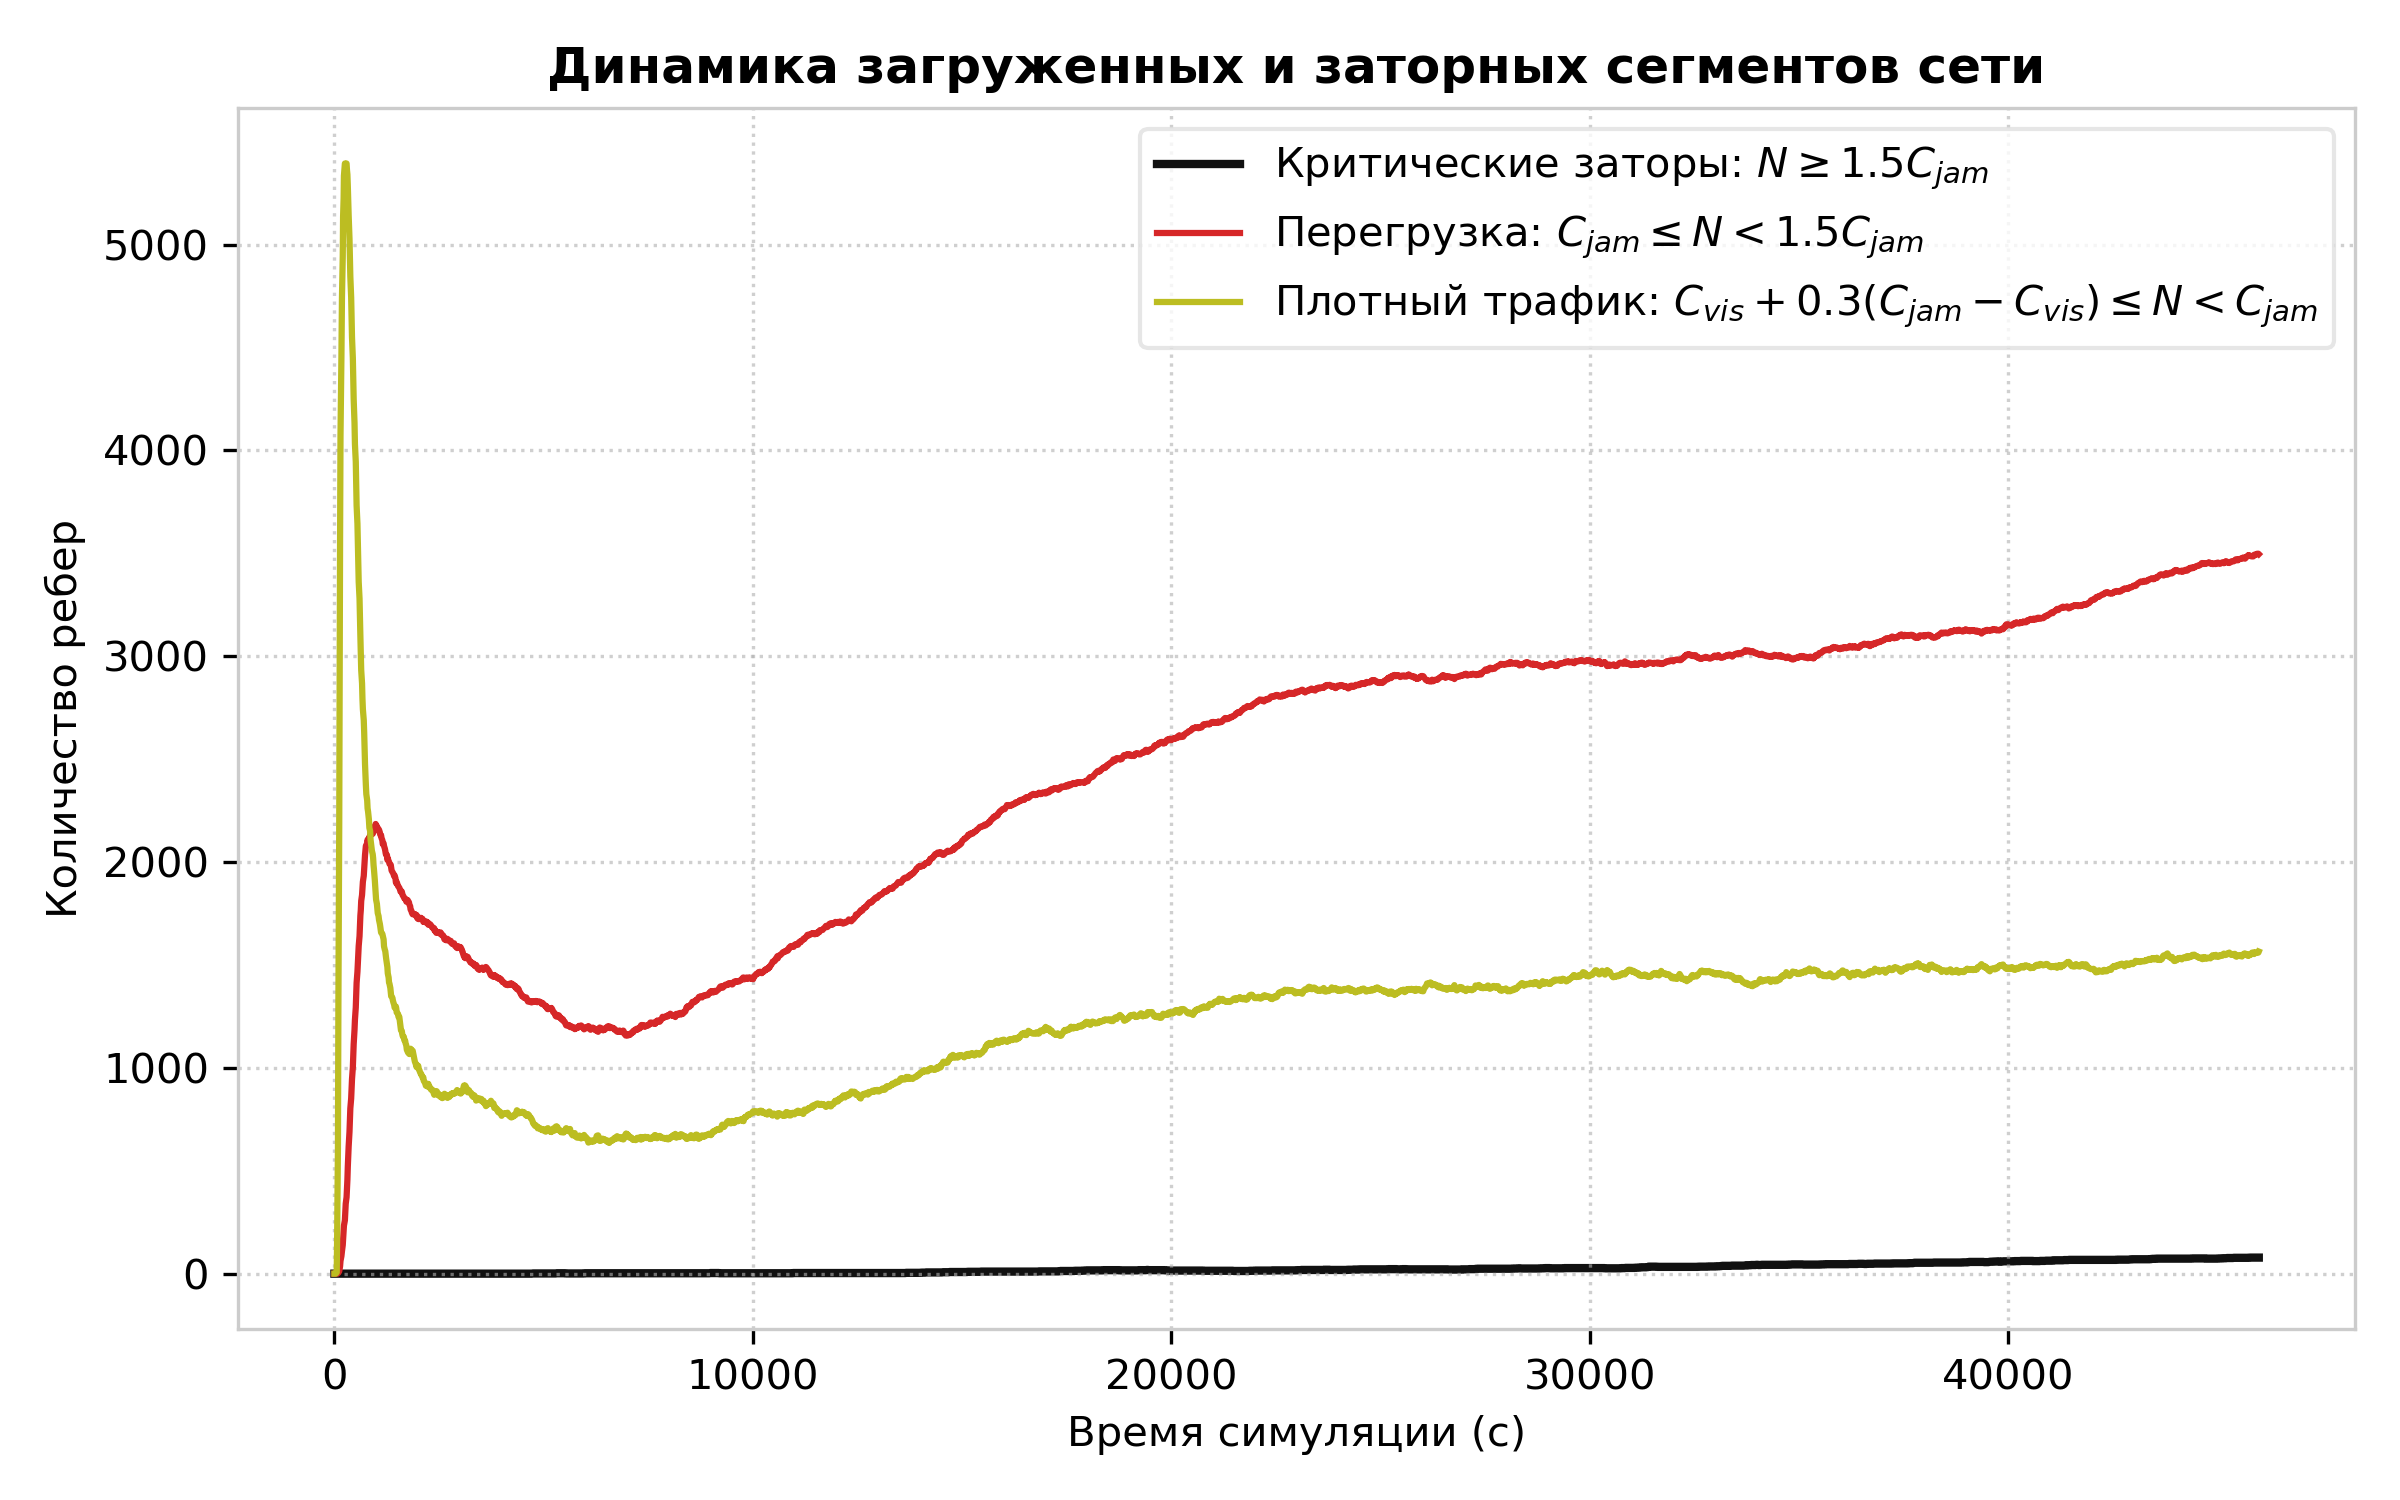
\includegraphics[width=0.85\linewidth,keepaspectratio]{assets/images/fig_red_yellow_zones.png}
    \caption{Динамика загруженных (желтых), перегруженных (красных) и заторных (черных) сегментов сети}
    \label{fig:sim_red_yellow_zones}
\end{figure}

Динамика очередей ожидания маршрутов приведена на рис. \ref{fig:sim_queues}. Очередь выпуска (первичный и повторный старт автомобилей) достигает пика в $81$~тыс. к $7000$~с, снижаясь до $4$~тыс. к концу симуляции. Очередь смены маршрута (запросы на перестроение пути во время движения) достигает максимума в $34$~тыс. к $17~000$~с и стабилизируется на уровне $26$~тыс. машин.

Показатели производительности ядра маршрутизации подтверждают эффективность системы. Средняя скорость обработки запросов (QPS) возрастает с $200$ до $500$ к $8~000$~с, испытывает кратковременное снижение до $400$--$450$ QPS на $11~000$~с (в период перестроения маршрутов), после чего возрастает до пика в $1050$ QPS к концу симуляции. Количество посещенных вершин при поиске пути $A^*$ пикует на уровне $210$ тыс. на $1000$~с, снижаясь до $50$ тыс. вершин к концу симуляции. Среднее время поиска пути снижается с $35$~мс до $9$~мс, хотя максимальное время расчета на сложных маршрутах сохраняет единичные выбросы в диапазоне $100$--$350$~мс. Данные показатели подтверждают, что вычислительное ядро справляется с нагрузкой, а расходимость модели носит транспортно-физический характер.

\begin{figure}[htbp]
    \centering
    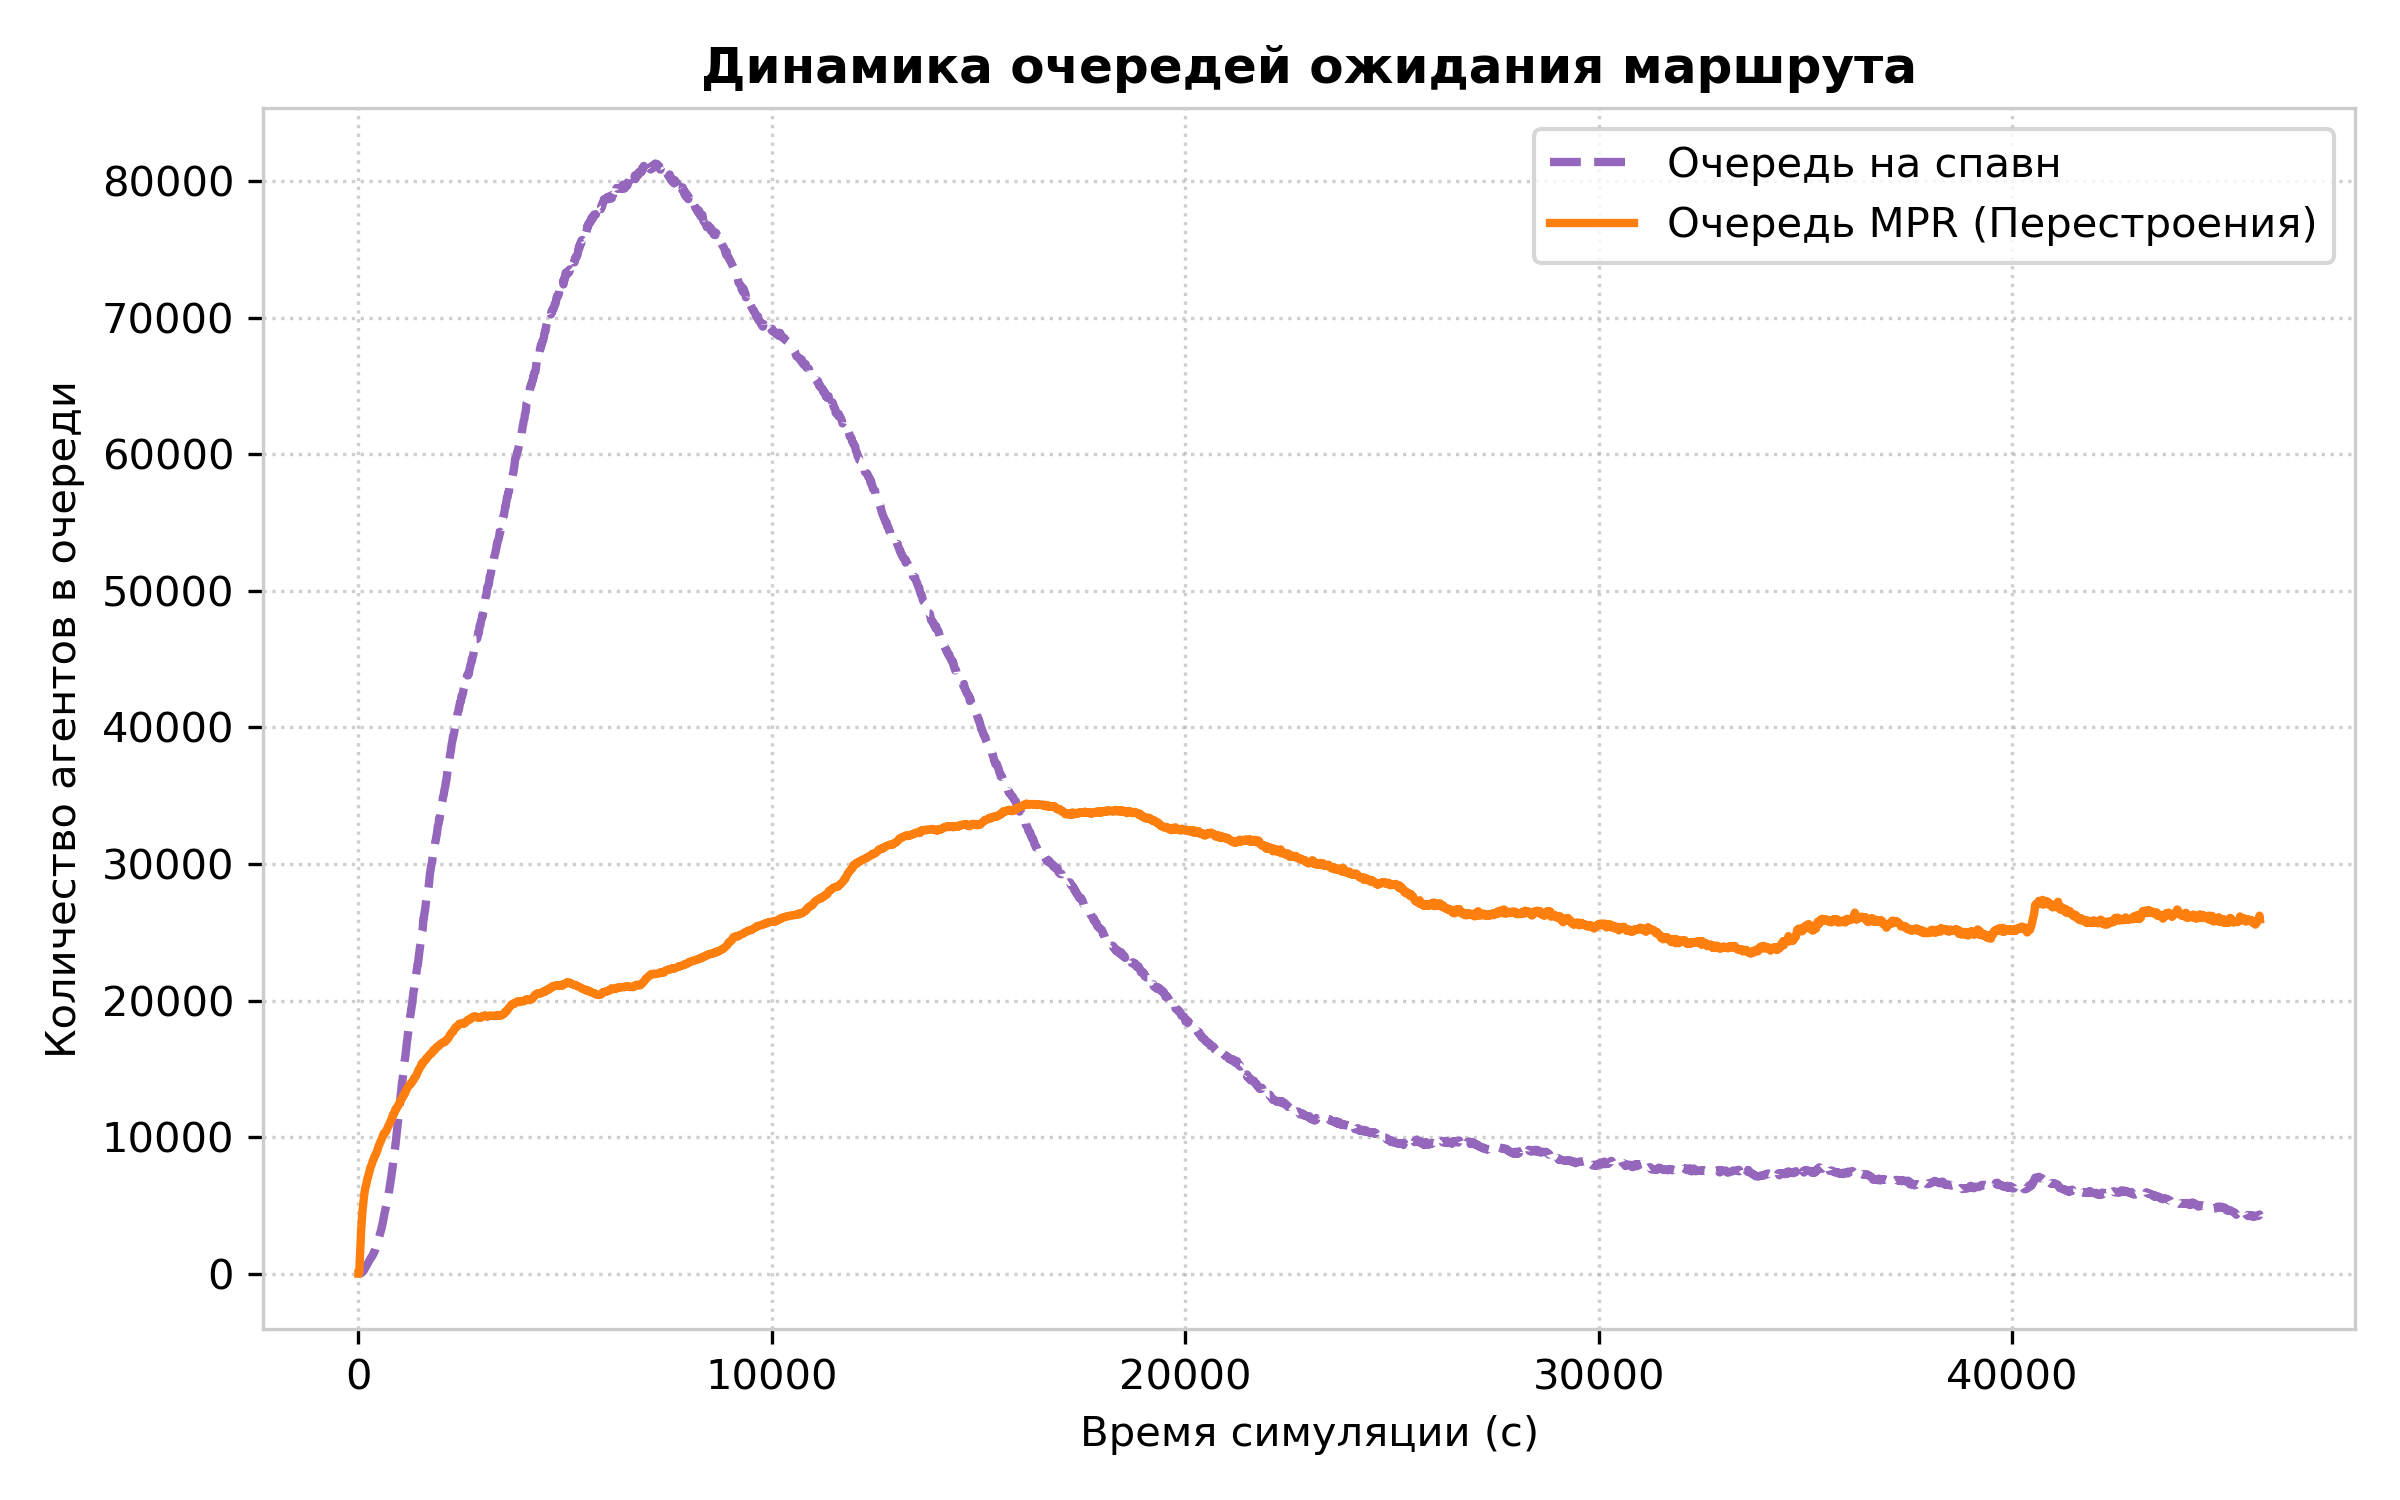
\includegraphics[width=0.85\linewidth,keepaspectratio]{assets/images/fig_queues.png}
    \caption{Динамика очередей ожидания маршрута (первичное появление и перестроения)}
    \label{fig:sim_queues}
\end{figure}

\section{Выводы по третьей главе}
Разработанные низкоуровневые алгоритмы поиска пути и архитектура ядра маршрутизации проверены в ходе экспериментов на субграфе Московской агломерации ($582$~тыс. узлов, $1~460$~тыс. рёбер). Применение метода ориентиров в связке с $8$-арной кучей ускорило поиск пути до $17{,}70$ раз по сравнению с базовым алгоритмом Дейкстры. Привязка потоков к ядрам процессора обеспечила скорость в $5130$ запросов в секунду при работе на $12$ потоках.

Однако интеграционный эксперимент выявил неустойчивость чисто реактивной маршрутизации в условиях запаздывания информации. Полученный отрицательный результат (отсутствие стабилизации TTI) обладает высокой научной ценностью: он строго очерчивает ограничения мезоскопического подхода и доказывает необходимость перехода от реактивного поиска к упреждающему регулированию. В качестве дальнейших направлений исследования предлагается внедрение механизмов мягких штрафов за транзит через потенциально перегружаемые сегменты дорожной сети и алгоритмов распределенной координации потоков на базе графовых нейронных сетей.

